\documentclass[aspectratio=169, 11pt]{beamer}

\makeatletter
\def\input@path{{./theme/}}
\makeatother
\graphicspath{{./theme/}}
\usetheme[cornerlogo=fullcolor, titlepagelogo=fullcolor, textcolor=blue, titlelayout=leftrule, monogram=none]{NotreDame}

\usepackage[T1]{fontenc}
\usepackage{lmodern}
\usepackage{booktabs}
\usepackage{listings}
\usepackage{tikz}
\usepackage{qrcode}
\usetikzlibrary{positioning, arrows.meta, calc, decorations.pathreplacing}
\usepackage{xcolor}

\definecolor{OkGreen}{HTML}{009E73}
\definecolor{OkVermillion}{HTML}{D55E00}
\definecolor{Muted}{HTML}{7A7A7A}
\definecolor{CodeBg}{HTML}{F4F4F2}

\tikzset{
  nd box/.style={draw=NDGold, line width=0.8pt, text=NDBlue,
    rounded corners=2pt, fill=white, align=center},
  nd highlight/.style={nd box, draw=IrishGreen}
}

\setbeamertemplate{navigation symbols}{}

\setbeamercolor{enumerate item}{fg=IrishGreen}
\setbeamercolor{enumerate subitem}{fg=IrishGreen}
\setbeamercolor{item projected}{bg=IrishGreen}

\newcommand{\good}[1]{\textcolor{OkGreen}{\ensuremath{\checkmark}~#1}}
\newcommand{\bad}[1]{\textcolor{OkVermillion}{\ensuremath{\times}~#1}}
\newcommand{\unknown}[1]{\textcolor{Muted}{?~#1}}

\newcommand{\slidepoint}[1]{{\large\color{NDBlue}#1}}

\lstdefinestyle{plain}{
  basicstyle=\ttfamily\scriptsize,
  backgroundcolor=\color{CodeBg},
  keywordstyle=\color{NDBlue}\bfseries,
  commentstyle=\color{Muted}\itshape,
  stringstyle=\color{IrishGreen},
  frame=leftline, framerule=1.2pt, rulecolor=\color{NDGold},
  framexleftmargin=4pt, xleftmargin=6pt,
  breaklines=true, showstringspaces=false,
  aboveskip=0.6em, belowskip=0.4em,
}
\lstset{style=plain}

\newcommand{\actstrip}[1]{%
\begin{tikzpicture}[x=3.1cm, font=\large\sffamily]
  \foreach \n [count=\i from 1] in {Tinker, Understand, Build, Challenge, Trust} {
    \pgfmathparse{int(\i == #1)}
    \ifnum\pgfmathresult=1
      \node[nd highlight,
            inner sep=6pt, minimum width=2.6cm, align=center] at (\i,0) {\textbf{\n}};
    \else
      \node[nd box,
            inner sep=6pt, minimum width=2.6cm, align=center] at (\i,0) {\n};
    \fi
    \ifnum\i<5
      \draw[-{Stealth[length=10pt]}, Muted, very thick]
        ($(\i,0)+(1.35cm,0)$) -- ($(\i,0)+(1.75cm,0)$);
    \fi
  }
\end{tikzpicture}}

\newcommand{\workspacesidebar}[1]{%
\begin{tikzpicture}[font=\small\sffamily]
  \foreach \n [count=\i from 1] in {Desktop app, Editor extension, Terminal} {
    \pgfmathparse{int(\i == #1)}
    \ifnum\pgfmathresult=1
      \node[nd highlight, inner sep=4pt, minimum width=2.8cm, align=center] at (0,-\i*1.0cm) {\textbf{\n}};
    \else
      \node[nd box, draw=Muted!45, text=Muted, inner sep=4pt, minimum width=2.8cm, align=center] at (0,-\i*1.0cm) {\n};
    \fi
  }
\end{tikzpicture}}

\newcommand{\stagedivider}[3]{%
\begin{frame}[plain]
  \vfill
  \begin{center}
    \actstrip{#1}\\[1.6em]
    {\LARGE\color{NDBlue}\textbf{#2}}\\[0.7em]
    {\large#3}
  \end{center}
  \vfill
\end{frame}}

% Transition slide for the six tasks: \taskdivider{n} shows task n in full ND Blue and the
% other five at 50% opacity. \taskrow{current}{this}{label} draws one row.
\newcommand{\taskrow}[3]{%
  \ifnum#1=#2
    \node[circle, fill=NDBlue, text=white, minimum size=0.72cm, inner sep=0pt] at (0,-#2*0.9cm) {\textbf{#2}};
    \node[anchor=west, text=NDBlue] at (0.75cm,-#2*0.9cm) {\textbf{#3}};
  \else
    \node[circle, draw=NDBlue, text=NDBlue, opacity=0.5, minimum size=0.72cm, inner sep=0pt] at (0,-#2*0.9cm) {#2};
    \node[anchor=west, text=NDBlue, opacity=0.5] at (0.75cm,-#2*0.9cm) {#3};
  \fi}

\newcommand{\taskdivider}[1]{%
\begin{frame}[plain]
  \vfill
  \begin{center}
    {\LARGE\color{NDBlue}\textbf{Six common scholarly tasks}}\\[0.4em]
    \begin{tikzpicture}[font=\large\sffamily]
      \taskrow{#1}{1}{Set up an agent workspace and inherit a project}
      \taskrow{#1}{2}{Convert code from a paper into a package}
      \taskrow{#1}{3}{Go from an idea to a literature review, report, or proposal}
      \taskrow{#1}{4}{Audit a manuscript before submission}
      \taskrow{#1}{5}{Draft a manuscript from the previous tasks}
      \taskrow{#1}{6}{Modernize a graduate course}
    \end{tikzpicture}
  \end{center}
  \vspace{0.8cm plus 1fill}
\end{frame}}

\title{Claude (or Codex) for Research}
\providecommand{\seminarpart}{0}
\author{Prof. Alexander (Alex) Dowling}
\institute{Chemical and Biomolecular Engineering \\ adowling@nd.edu}
\date{28 September 2026 \quad$\vert$\quad 12 October 2026}
\ndvenue{McCourtney Hall B01 Auditorium}

\renewcommand{\ndcornerlogoheight}{0.839cm}
\renewcommand{\ndcornerlogomargin}{0.5mm}

\renewcommand{\ndlogonoteanchor}{0.518}

\newcommand{\sessiontitle}[3]{%
  \part{#1}
  \subtitle{Beyond the Chatbot}
  \date{#3}
  {
  \setbeamertemplate{background}{\ndtitlepagelogodraw}
  \begin{frame}[plain]
    \titlepage
    \begin{tikzpicture}[remember picture,overlay]
      \node[anchor=north west, text=NDBlue, font=\large]
        at ([xshift=0.25cm,yshift=-2.65cm]current page.north west) {\textbf{#1: #2}};
    \end{tikzpicture}
  \end{frame}
  }
}

\providecommand{\partoneregroup}{}
\providecommand{\parttworegroup}{}

\begin{document}

% part1_slides.tex and part2_slides.tex select one part. A part number of 0 would
% build both in one sequence; no make target uses it.
\ifnum\seminarpart=2\else
  \sessiontitle{Part 1}{Setting up a project}{28 September 2026}
  \begin{frame}{Creating faculty-visitor schedules for graduate student recruitment}
  \ndlogonote{\scriptsize\href{https://github.com/dowlinglab/grad-visit-scheduler}{\texttt{github.com/dowlinglab/grad-visit-scheduler}}}
  \vfill
  \begin{columns}[c]
    \begin{column}{0.50\textwidth}
      \centering
      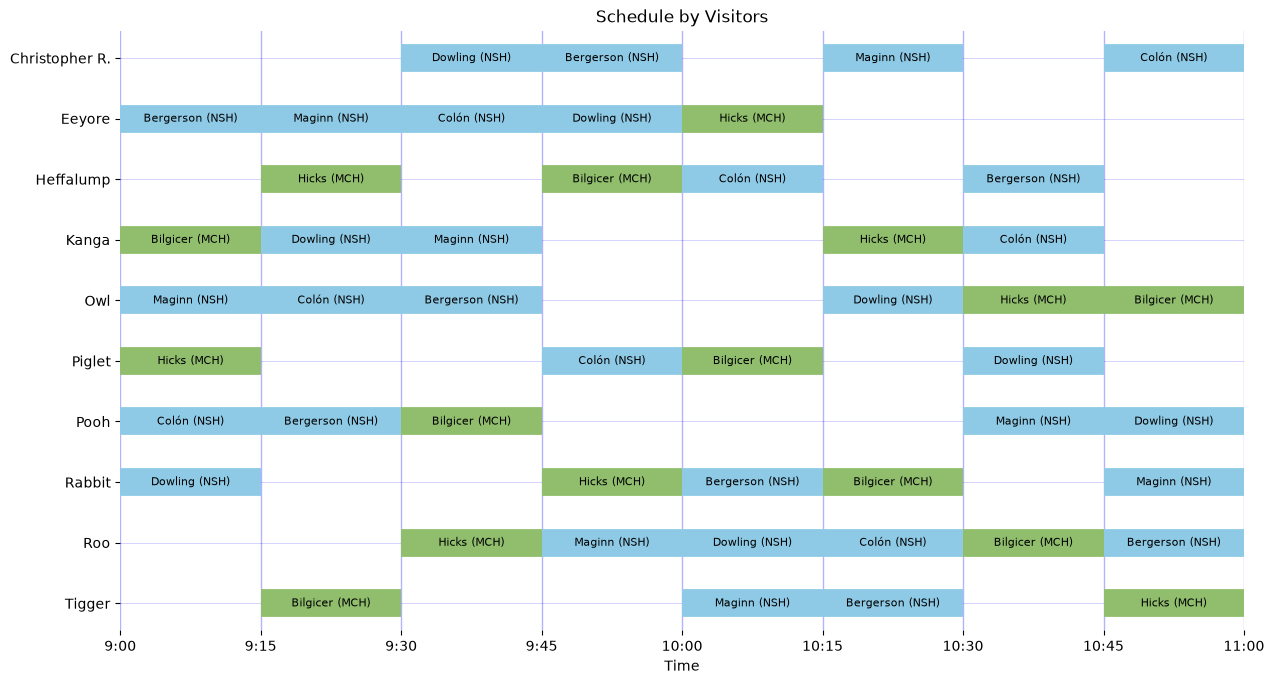
\includegraphics[width=\linewidth,height=5.9cm,keepaspectratio]{figures/grad_visit_schedule_10}
    \end{column}
    \begin{column}{0.46\textwidth}
      \centering
      \resizebox{!}{5.9cm}{%
      \begin{tikzpicture}[font=\scriptsize, node distance=0.5cm]
        \node[nd box, minimum width=6.2cm, minimum height=1cm, text width=5.8cm, align=center]
          (a) {\textbf{Before 2023}\\DGA spent \textasciitilde10 hours (re)making the schedule by hand};
        \node[nd box, minimum width=6.2cm, minimum height=1cm, text width=5.8cm, align=center, below=of a]
          (b) {\textbf{2023}\\Jeff Kantor and I built a Jupyter notebook that used discrete optimization to create the schedule.};
        \node[nd box, minimum width=6.2cm, minimum height=1cm, text width=5.8cm, align=center, below=of b]
          (c) {\textbf{2024--2025}\\I maintained the notebook, patching it by hand, inputting data, and creating schedules each year.};
        \node[nd highlight, minimum width=6.2cm, minimum height=1cm, text width=5.8cm, align=center, below=of c]
          (d) {\textbf{Feb 2026}\\Using Codex, I converted the schedule optimization code into a tested, public Python package.};
        \draw[-{Stealth[length=6pt]}, thick] (a) -- (b);
        \draw[-{Stealth[length=6pt]}, thick] (b) -- (c);
        \draw[-{Stealth[length=6pt]}, thick] (c) -- (d);
      \end{tikzpicture}}
    \end{column}
  \end{columns}
  \vspace{0.7cm plus 1fill}
\end{frame}

\begin{frame}[fragile]{Jupyter Notebook $\to$ public Python package in \textasciitilde10 hours}
  \ndlogonote{\scriptsize\href{https://grad-visit-scheduler.readthedocs.io}{\texttt{grad-visit-scheduler.readthedocs.io}}}
  \begin{columns}[T]
    \begin{column}{0.46\textwidth}
      \begin{minipage}[t]{\linewidth}
      \centering
      \scriptsize
      \renewcommand{\arraystretch}{0.82}
      \begin{tabular}{@{}lll@{}}
        \toprule
        \textbf{Ver.} & \textbf{Date} & \textbf{What changed} \\
        \midrule
        \texttt{---} & Feb 9 & Draft 1 of 2026 schedule \\
        \texttt{---} & Feb 9 & notebook $\to$ tested pkg \\
        \texttt{v0.1.1} & Feb 10 & Initial public release \\
        \texttt{v0.2.0} & Feb 13 & Top-N schedules \\
        \texttt{v0.3.0} & Feb 13 & Multi-building, travel time \\
        \texttt{v0.3.1} & Feb 17 & Full tests, docs complete \\
        \texttt{v0.4.0} & Feb 25 & Hard constraints (advanced API) \\
        \texttt{v0.5.0} & Mar 11 & Separate faculty/student breaks \\
        \texttt{v0.5.1} & Sep 4 & Auto-sized plots \\
        \bottomrule
      \end{tabular}
      \end{minipage}
    \end{column}
    \begin{column}{0.5\textwidth}
      \begin{minipage}[t]{\linewidth}
      \centering
      
\includegraphics[width=\linewidth]{figures/grad_scheduler_screenshot_crop}
      \end{minipage}
    \end{column}
  \end{columns}
  \vspace{0.3em}
  \begin{center}\small
    On sabbatical this past February, I nearly said no. Then, I used this project to test Codex.
  \end{center}
  \vspace{0.2em}
  \begin{center}\small
    After this small project, I got everyone in my group an \textbf{ND OpenAI seat}. We regularly discuss \textbf{AI best wins, traps, and practices} in our weekly group meeting.
  \end{center}
  \vspace{0.7cm plus 1fill}
\end{frame}

\begin{frame}{Takeaway message for today}
  \vfill
  \begin{center}
    \slidepoint{The most powerful uses of generative AI in research go beyond\\
    asking a chatbot questions or polishing prose.}
  \end{center}
  \vspace{1.2em}
  \begin{center}
    \slidepoint{They come from putting AI inside a workflow that is\\
    \textbf{deliberate, reproducible, and auditable}.}
  \end{center}
  \vfill
\end{frame}

  
\begin{frame}{Borrowed structure}
  \vfill
  \begin{columns}[c]
    \begin{column}{0.54\textwidth}
      \centering
      \large
      \begin{tabular}{@{}l@{\hspace{0.5cm}}l@{}}
        \textbf{Part 1} & \color{NDGold!80!black}\textbf{Prologue:} \textbf{\color{NDBlue}Tinker} \\[0.8em]
        & \color{NDGold!80!black}\textbf{Act I:} \textbf{\color{NDBlue}Understand} {\small\color{NDBlue}(Task 1)} \\[0.8em]
        & \color{NDGold!80!black}\textbf{Act II:} \textbf{\color{NDBlue}Build} {\small\color{NDBlue}(Task 2)} \\[1.1em]
        \textbf{Part 2} & \color{NDGold!80!black}\textbf{Act II:} \textbf{\color{NDBlue}Build} {\small\color{NDBlue}(Task 3)} \\[0.8em]
        & \color{NDGold!80!black}\textbf{Act III:} \textbf{\color{NDBlue}Challenge} {\small\color{NDBlue}(Tasks 4--6)} \\[0.8em]
        & \color{NDGold!80!black}\textbf{Epilogue:} \textbf{\color{NDBlue}Trust}
      \end{tabular}
    \end{column}
    \begin{column}{0.42\textwidth}
      \centering
      
\includegraphics[width=0.62\textwidth]{figures/tal_logo}\\[1.1em]
      {\small\itshape%
        We will borrow the three-act format.\\[0.8em]
        But to temper expectations, I am not as entertaining as Ira Glass.}
    \end{column}
  \end{columns}
  \vfill
\end{frame}

  
\begin{frame}{Today: my lessons learned and recommended practices}
  \vfill
  \begin{columns}[t]
    \begin{column}{0.48\textwidth}
      \textbf{This is not}
      \begin{itemize}
        \item a Claude tutorial
        \item a Claude vs.\ Codex throw down
        \item a claim that AI does research
      \end{itemize}
    \end{column}
    \begin{column}{0.48\textwidth}
      \textbf{This is}
      \begin{itemize}
        \item lessons from one year of use, including failures
        \item mostly model-independent practices
        \item changes you can make tomorrow
      \end{itemize}
    \end{column}
  \end{columns}
  \vspace{0.8em}
  \begin{center}
    \textbf{My past year, distilled into six research task types}\\[0.6em]
    \small
    \begin{tabular}{@{}l@{\hspace{0.8cm}}l@{\hspace{0.9cm}}l@{}}
      \textbf{\color{NDGold!80!black}Part 1} & 1.~Set up agents and inherit a project & 2.~Paper code $\to$ public package \\[0.7em]
      \textbf{\color{NDGold!80!black}Part 2} & 3.~Idea $\to$ literature review, report, or proposal & 4.~Audit a manuscript \\[0.55em]
      & 5.~Project $\to$ manuscript & 6.~Modernize a course \\
    \end{tabular}
  \end{center}
  \vfill
\end{frame}

\begin{frame}{Which model, and how much of it do you get}
  \vfill
  \begin{center}
  \begin{tabular}{@{}lll@{}}
    \toprule
    & \textbf{Frontier models, small $\to$ large} & \textbf{Usage meter} \\
    \midrule
    Anthropic & Haiku 4.5, Sonnet 5, Opus 5, Fable 5.1 & 5-hour session + weekly cap \\
    OpenAI & GPT-5.6 Luna, Terra, Sol & 5-hour + weekly windows* \\
    & GPT-6 Luna, Sol, Astra & \\
    \bottomrule
  \end{tabular}
  \end{center}
  \vspace{0.5em}
  \begin{center}
    {\scriptsize * OpenAI limits vary by plan.}
  \end{center}
  \vspace{1.0em}
  \begin{center}
    \slidepoint{The mid-tier model (\textbf{Sonnet}, \textbf{Sol}) is usually the \textbf{right default}. Save Astra or Fable for the hardest work.}
  \end{center}
  \vfill
\end{frame}

\begin{frame}[fragile]{Everything today is on GitHub}
  \ndlogonote{\scriptsize\href{https://github.com/dowlinglab/claude-for-researchers}{\texttt{github.com/dowlinglab/claude-for-researchers}}}
  \vfill
  \vspace{-0.75cm}
  \begin{columns}[t]
    \begin{column}{0.46\textwidth}
      {\small\textbf{practices/} \scriptsize(10 -- guides)}
      \begin{itemize}\scriptsize\setlength\itemsep{0.15em}
        \item grant\_proposal\_writing
        \item latex\_overleaf\_workflow
        \item literature\_review
        \item manuscript\_audit
        \item private\_code\_to\_public\_package
        \item scientific\_computing\_workflow
        \item scientific\_figures\_tables
        \item technical\_writing
        \item working\_with\_ai\_agents
        \item writing\_style\_guide
      \end{itemize}
      \vspace{0.25em}
      {\small\textbf{checklists/} \scriptsize(1 -- verify + hand off)}
      \begin{itemize}\scriptsize\setlength\itemsep{0.15em}
        \item reproducibility\_and\_handoff\_checklist
      \end{itemize}
    \end{column}
    \begin{column}{0.5\textwidth}
      {\small\textbf{prompts/} \scriptsize(5 -- ready to paste in)}
      \begin{itemize}\scriptsize\setlength\itemsep{0.15em}
        \item literature\_workflow
        \item manuscript\_audit
        \item organize\_research\_repo
        \item proposal\_review
        \item getting\_started
      \end{itemize}
      \vspace{0.5em}
      {\small\textbf{scripts/} \scriptsize(4 -- tools)}
      \begin{itemize}\scriptsize\setlength\itemsep{0.15em}
        \item check\_docs.py
        \item doi\_checker
        \item figure\_style
        \item latexdiff\_check.sh
      \end{itemize}
      \vspace{0.5em}
      {\small\textbf{templates/} \scriptsize(3 -- fill in and go)}
      \begin{itemize}\scriptsize\setlength\itemsep{0.15em}
        \item project\_entry\_point
        \item research\_log
        \item results\_manifest
      \end{itemize}
    \end{column}
  \end{columns}
  \vspace{0.75cm}
  \vfill
\end{frame}

  \stagedivider{2}{Act I: Understand}{Set up the workspace for reproducible work}

\begin{frame}{An agent works on your file system}
  \vfill
  \begin{center}
  \begin{tikzpicture}[font=\normalsize, node distance=1.3cm]
    \node[nd box, minimum width=3.1cm, minimum height=1.6cm, align=center]
      (a) {\textbf{LLM}\\\small the model};
    \node[nd box, minimum width=3.9cm, minimum height=1.6cm, align=center, right=of a]
      (b) {\textbf{Chatbot}\\\small conversation + attachments};
    \node[nd highlight, minimum width=4.2cm, minimum height=1.6cm, align=center, right=of b]
      (c) {\textbf{Agent}\\\small model + tools + workspace};
    \draw[-{Stealth[length=6pt]}, thick] (a) -- (b);
    \draw[-{Stealth[length=6pt]}, thick] (b) -- (c);
  \end{tikzpicture}
  \end{center}
  \vspace{0.7em}
  \begin{center}
    An agent can inspect the real files, edit them, \textbf{run code and tests}, search Git history, and \textbf{commit and push to Git}.
  \end{center}
  \vspace{0.6em}
  \begin{center}
    \slidepoint{The useful shift is from describing a project to letting an agent inspect it.}
  \end{center}
  \vfill
\end{frame}

\begin{frame}{Use version control with (almost) every agentic project}
  \ndlogonote{\scriptsize Getting started: \href{https://github.com/education}{\texttt{github.com/education}}\quad\href{https://youtu.be/a9u2yZvsqHA}{tutorial}\quad\href{https://desktop.github.com/download}{\texttt{desktop.github.com/download}}}
  \vspace{-0.45cm}
  \begin{columns}[t]
    \begin{column}{0.30\textwidth}
      {\centering\textbf{A conversation}\\[0.15em]
        {\footnotesize\color{Muted}good}\par}
      \vspace{0.5em}
      \begin{itemize}\footnotesize\setlength\itemsep{0.22em}
        \item you paste context in and copy results out
        \item tied to one session
        \item difficult to share or search
        \item disappears with the tool
      \end{itemize}
    \end{column}
    \begin{column}{0.30\textwidth}
      {\centering\textbf{A file system}\\[0.15em]
        {\footnotesize\color{NDGold!80!black}better}\par}
      \vspace{0.5em}
      \begin{itemize}\footnotesize\setlength\itemsep{0.22em}
        \item the agent reads and edits the real files
        \item no copy-paste step
        \item every change overwrites what was there
        \item one bad edit is unrecoverable
      \end{itemize}
    \end{column}
    \begin{column}{0.30\textwidth}
      {\centering\textbf{\color{NDBlue}A repository}\\[0.15em]
        {\footnotesize\color{IrishGreen}\textbf{best}}\par}
      \vspace{0.5em}
      \begin{itemize}\footnotesize\setlength\itemsep{0.22em}
        \item every change is saved and labeled
        \item searchable history
        \item compare versions and recover
        \item survives tools, people, and computers
      \end{itemize}
    \end{column}
  \end{columns}
  \vspace{1.1em}
  \begin{center}\small
    \textbf{Version control} keeps a dated record of every saved change. Use it for every
    research project you share: when an agent breaks something, Git is how you undo it.
  \end{center}
  \vspace{0.9cm plus 1fill}
\end{frame}

\begin{frame}{Desktop app: supervise several tasks at once}
  \ndlogonote{\scriptsize Screenshot: Claude desktop; other project names blurred}
  \vfill
  \begin{columns}[c,onlytextwidth]
    \begin{column}{0.22\textwidth}
      \centering\workspacesidebar{1}\par
      \vspace{0.65cm}
      \raggedright\small\color{NDBlue}No setup. I use it more than \textbf{90\%} of the time.
    \end{column}
    \begin{column}{0.76\textwidth}
      \centering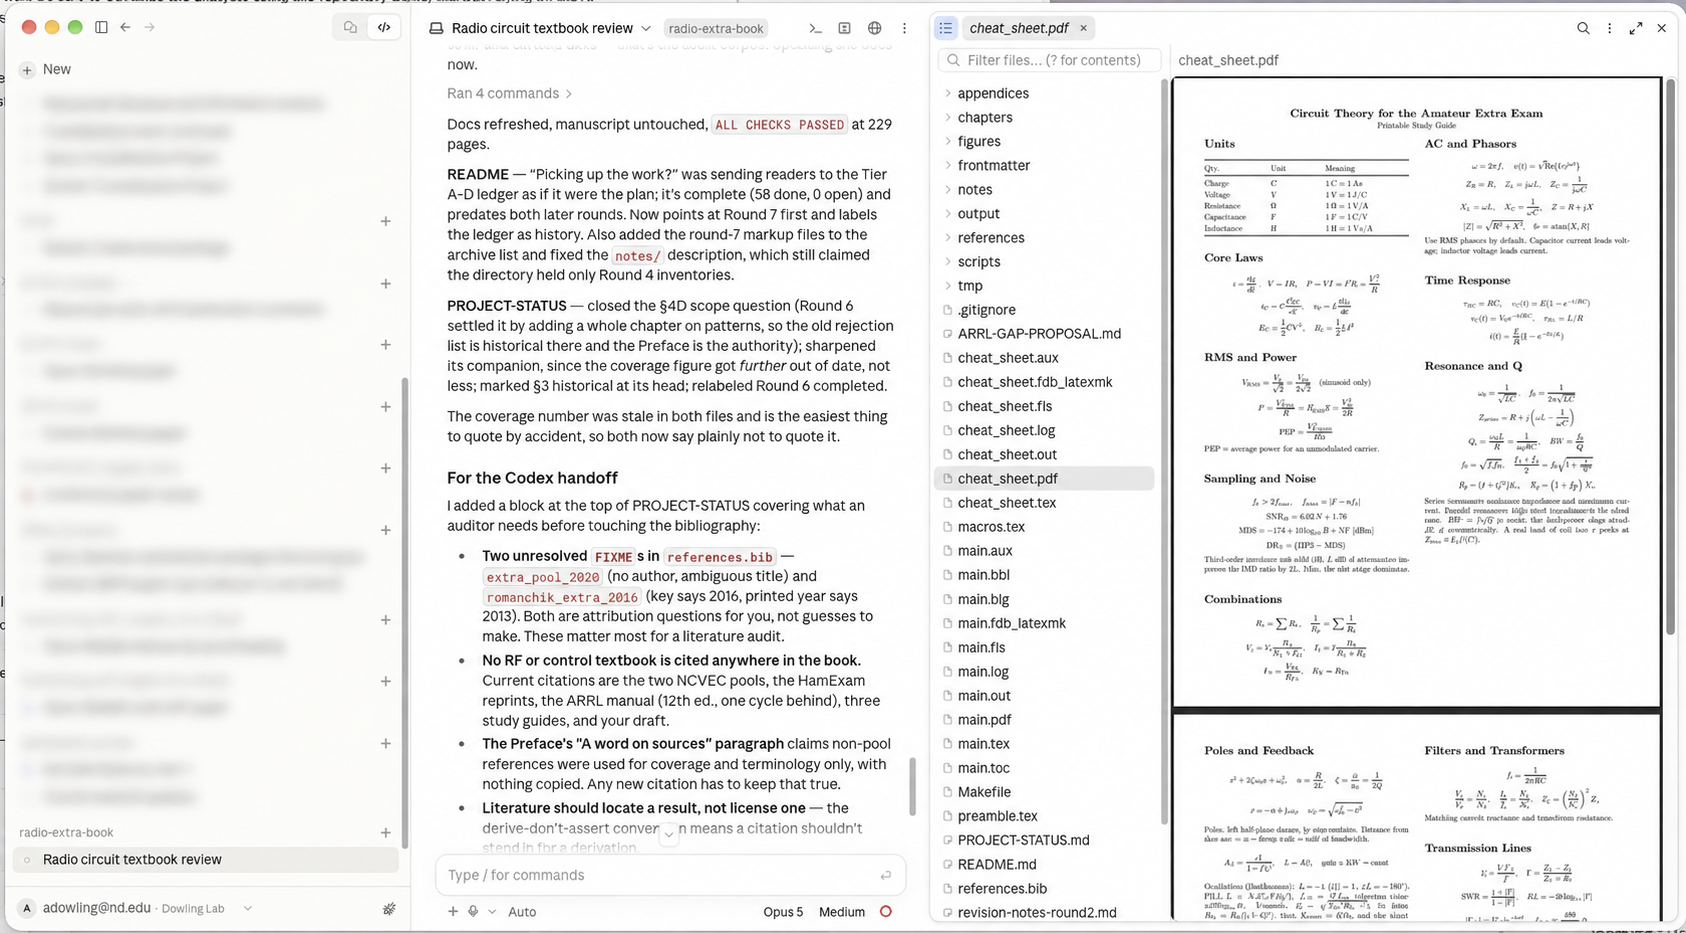
\includegraphics[width=\linewidth,height=5.4cm,keepaspectratio]{figures/claude_desktop_projects_blurred.png}
    \end{column}
  \end{columns}
  \vfill
\end{frame}

\begin{frame}{Editor extension: a tight edit-review loop}
  \ndlogonote{\scriptsize Screenshot: \href{https://code.claude.com/docs/en/vs-code}{Claude Code documentation}}
  \vfill
  \begin{columns}[c,onlytextwidth]
    \begin{column}{0.22\textwidth}
      \centering\workspacesidebar{2}\par
      \vspace{0.65cm}
      \raggedright\small\color{NDBlue}Best when you are already reading the code.
    \end{column}
    \begin{column}{0.76\textwidth}
      \centering
      \begin{tikzpicture}
        \node[anchor=south west, inner sep=0] (img) at (0,0)
          {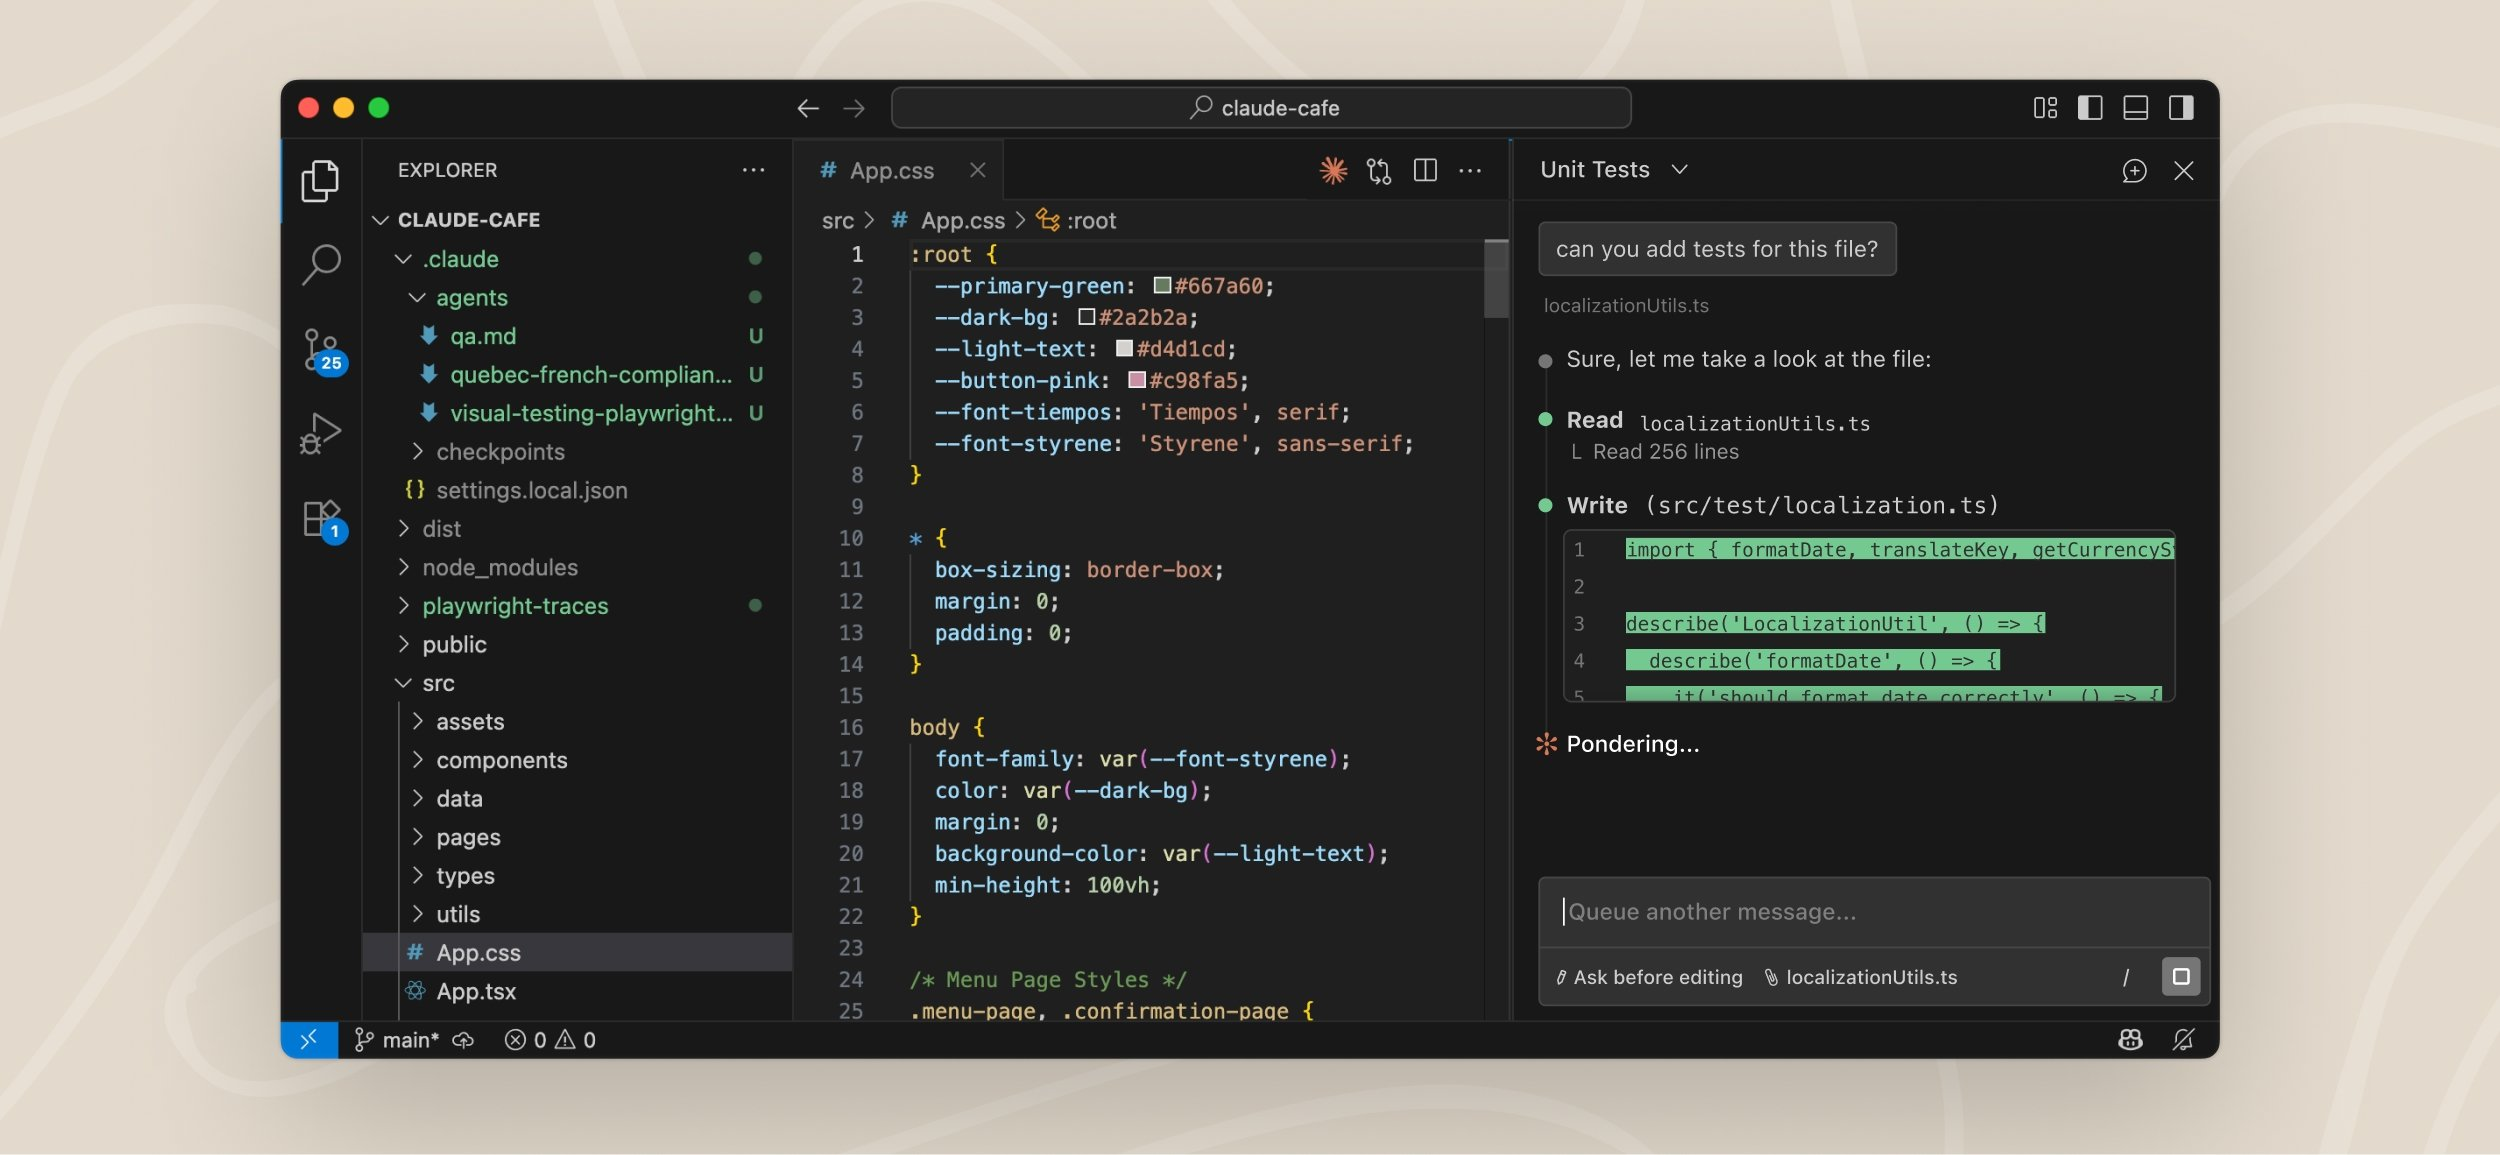
\includegraphics[width=\linewidth,height=5.4cm,keepaspectratio]{figures/claude_vscode_extension}};
        \begin{scope}[x={(img.south east)}, y={(img.north west)}]
          \node[fill=white, draw=NDGold, line width=0.7pt, rounded corners=1.5pt,
                inner sep=2.5pt, font=\scriptsize, text=NDBlue] (lbl) at (0.70,0.22)
            {proposed edit, inline};
          \draw[-{Stealth[length=5pt]}, NDGold, very thick] (lbl.north) -- (0.70,0.42);
        \end{scope}
      \end{tikzpicture}
    \end{column}
  \end{columns}
  \vfill
\end{frame}

\begin{frame}{Terminal: scriptable, and the same engine underneath}
  \ndlogonote{\scriptsize Screenshot: \href{https://code.claude.com/docs/en/agent-view}{Claude Code documentation}}
  \vfill
  \begin{columns}[c,onlytextwidth]
    \begin{column}{0.22\textwidth}
      \centering\workspacesidebar{3}\par
      \vspace{0.65cm}
      \raggedright\small\color{NDBlue}The only one you can put in \textbf{cron or CI}.
    \end{column}
    \begin{column}{0.76\textwidth}
      \centering
      \begin{tikzpicture}
        \node[anchor=south west, inner sep=0] (img) at (0,0)
          {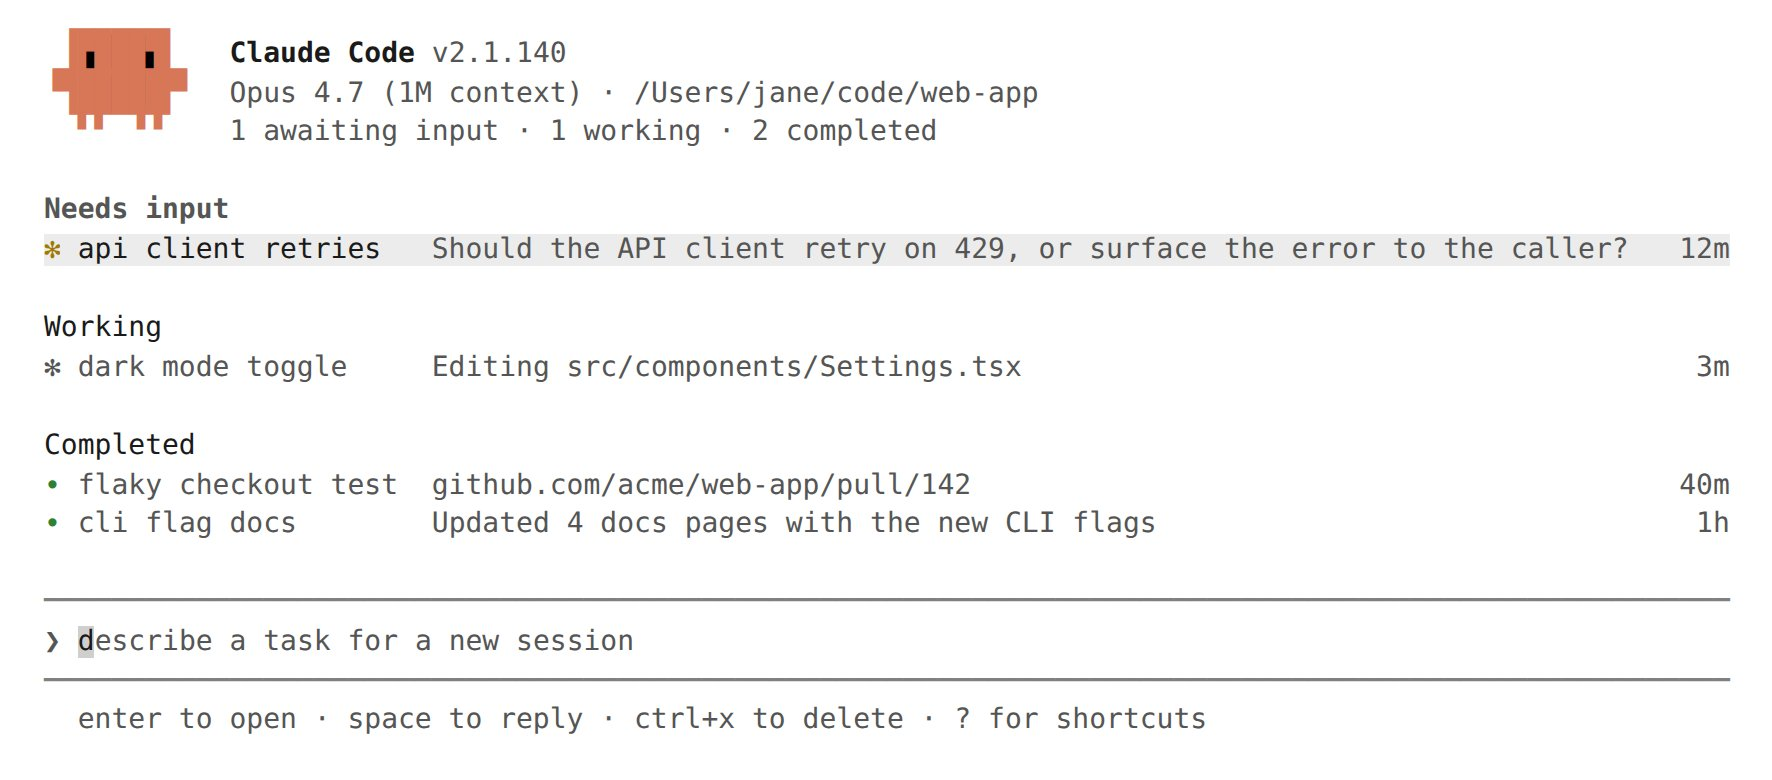
\includegraphics[width=\linewidth,height=5.4cm,keepaspectratio]{figures/claude_terminal_agent_view}};
        \begin{scope}[x={(img.south east)}, y={(img.north west)}]
          \node[fill=white, draw=NDGold, line width=0.7pt, rounded corners=1.5pt,
                inner sep=2.5pt, font=\scriptsize, text=NDBlue] (lbl) at (0.82,0.93)
            {sessions grouped by state};
          \draw[-{Stealth[length=5pt]}, NDGold, very thick] (lbl.west) -- (0.49,0.86);
        \end{scope}
      \end{tikzpicture}
    \end{column}
  \end{columns}
  \vfill
\end{frame}

\taskdivider{1}

\begin{frame}{Task 1: Inherit a project from a colleague}
  \vfill
  \begin{center}
  \begin{tikzpicture}
    \node[nd box, text width=10.6cm, align=left, inner sep=0.45cm] {%
      \small\itshape
      Welcome to the group. You are taking over this project from a
      student who graduated last spring.\\[0.5em]
      Here is a zip file with what I think is the most recent code, and
      here is our latest paper.\\[0.5em]
      Figure out how to reproduce the results in the paper using this
      code. Then we can extend it.};
  \end{tikzpicture}
  \end{center}
  \vspace{0.9em}
  \begin{center}\small
    No repository. No environment file. No record of which script made which figure.
  \end{center}
  \vspace{0.5em}
  \begin{center}
    \slidepoint{Before you can extend the work, you have to be able to \textbf{rerun} it.}
  \end{center}
  \vspace{0.6cm plus 1fill}
\end{frame}

\begin{frame}{Task 1: Set up an agent workspace and inherit a project}
  \ndlogonote{\scriptsize\href{https://github.com/dowlinglab/claude-for-researchers/blob/main/resources/prompts/organize_research_repo.md}{\texttt{resources/prompts/organize\_research\_repo.md}}}
  \vfill
  \begin{enumerate}\setlength\itemsep{0.7em}
    \item \textbf{Configure version control}: initialize Git, connect GitHub, make a clean baseline commit.
    \item \textbf{Create the computing environment}: record dependencies, installation, and the commands that reproduce current results.
    \item \textbf{Configure the agents}: add project instructions, permissions, write boundaries, and verification commands.
    \item \textbf{Explore before editing}: inventory the files, run the easiest result, then map the workflow from inputs to outputs.
  \end{enumerate}
  \vfill
  \begin{center}
    \slidepoint{The first deliverable is a \textbf{reproducible baseline}, not a refactor.}
  \end{center}
  \vspace{1.2cm plus 1fill}
\end{frame}

\begin{frame}{Branches isolate a change; pull requests invite review}
  \ndlogonote{\scriptsize Screenshot: \href{https://docs.github.com/en/desktop/making-changes-in-a-branch/committing-and-reviewing-changes-to-your-project-in-github-desktop}{GitHub Docs}}
  \vfill
  \begin{columns}[c]
    \begin{column}{0.43\textwidth}
      \centering
      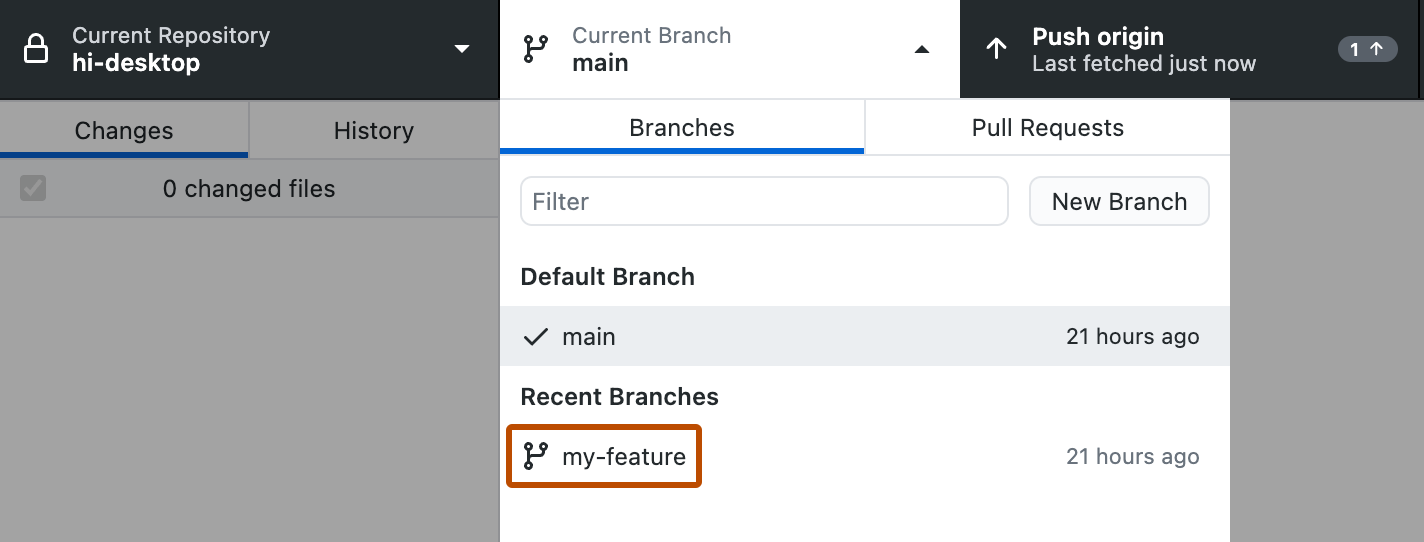
\includegraphics[width=0.94\linewidth,height=4.8cm,keepaspectratio]{figures/github_desktop_branch.png}
    \end{column}
    \begin{column}{0.52\textwidth}
      \begin{enumerate}\small\setlength\itemsep{0.9em}
        \item \textbf{Branch}: work on one feature or revision separately.
        \item \textbf{Pull request}: show collaborators the changes and checks.
        \item \textbf{Merge}: bring reviewed work back into the shared branch.
      \end{enumerate}
      \vspace{0.6em}
      \small Use separate branches for overlapping agent work. A branch isolates edits; it does not eliminate merge conflicts.
    \end{column}
  \end{columns}
  \vspace{0.8cm plus 1fill}
\end{frame}

\begin{frame}{Project instructions: \texttt{CLAUDE.md} and \texttt{AGENTS.md}}
  \ndlogonote{\scriptsize\href{https://github.com/dowlinglab/claude-for-researchers/blob/main/resources/practices/working_with_ai_agents.md}{\texttt{resources/practices/working\_with\_ai\_agents.md}}}
  \vfill
  \begin{center}\small
  \renewcommand{\arraystretch}{1.12}
  \begin{tabular}{@{}>{\raggedright\arraybackslash}p{2.7cm}>{\raggedright\arraybackslash}p{4.7cm}>{\raggedright\arraybackslash}p{4.7cm}@{}}
    \toprule
    & \textbf{Claude Code} & \textbf{Codex} \\
    \midrule
    Primary file & \texttt{CLAUDE.md} & \texttt{AGENTS.md} \\
    When read & at session start; nested files load when needed & before work starts; root-to-working-directory hierarchy \\
    Share one core & \texttt{CLAUDE.md} can import \texttt{AGENTS.md} & keep common rules in \texttt{AGENTS.md} \\
    Setup help & \texttt{/init} drafts; \texttt{/memory} inspects loaded files & \texttt{/init} drafts \texttt{AGENTS.md}; review and refine it \\
    \bottomrule
  \end{tabular}
  \end{center}
  \vspace{0.35em}
  \begin{center}
    \small Think of these as a \textbf{startup briefing}: project instructions added to context. They do not enforce permissions or guarantee compliance.
  \end{center}
  \vspace{0.5cm plus 1fill}
\end{frame}

\begin{frame}[fragile]{A concise instruction file routes the agent to evidence}
  \ndlogonote{\scriptsize\href{https://github.com/dowlinglab/claude-for-researchers/blob/main/resources/templates/project_entry_point.md}{\texttt{resources/templates/project\_entry\_point.md}}}
  \vfill
  \begin{columns}[c]
    \begin{column}{0.61\textwidth}
      \begin{lstlisting}[basicstyle=\ttfamily\scriptsize]
# Project
Estimate membrane transport parameters.
# Example: environment name is transport.

## Start here
- Model: src/
- Generated results: results/
- Decisions and dead ends: notes/log.md

## Verify changes
conda env create -f environment.yml
conda run -n transport python -m pytest

## Boundaries
- Never edit generated results by hand.
- Flag changes in numerical output.
      \end{lstlisting}
    \end{column}
    \begin{column}{0.35\textwidth}
      \small
      \textbf{Include}\par
      project map, setup commands, tests, conventions, and boundaries.\\[0.7em]
      \textbf{Keep elsewhere}\par
      detailed history, long plans, and background a tool can discover.\\[0.7em]
      \textbf{Improve from experience}\par
      recurring correction $\rightarrow$ concise rule or automated check.
    \end{column}
  \end{columns}
  \vspace{1.0cm plus 1fill}
\end{frame}

\begin{frame}[fragile]{Ask for help writing the task, not just the work}
  \ndlogonote{\scriptsize\href{https://github.com/dowlinglab/claude-for-researchers/blob/main/resources/practices/working_with_ai_agents.md}{\texttt{resources/practices/working\_with\_ai\_agents.md} \S12}}
  \vspace{-0.15cm}
  \begin{lstlisting}[basicstyle=\ttfamily\scriptsize]
I would like help developing a task that does the following.

I inherited a zip file of a former group member's code and the
paper it produced. Reproduce Figure 3 of that paper.

  1. Put the code in Git and make a baseline commit
  2. Infer the dependencies and build a clean environment
  3. Inventory the files and map inputs to outputs
  4. Run the easiest result first, then work up to Figure 3
  5. Record what reproduced, what failed, and what you skipped

Ask me questions before you write the task. For each step, say
what evidence proves it is finished and what you must leave to me.
  \end{lstlisting}
  \vspace{0.15em}
  \begin{center}
    \slidepoint{The first overnight prompt is about the \textbf{task}, not the work.}
  \end{center}
  \vspace{0.35cm plus 1fill}
\end{frame}

\begin{frame}{Then draft, review, launch, and explore}
  \ndlogonote{\scriptsize\href{https://github.com/dowlinglab/claude-for-researchers/blob/main/resources/practices/working_with_ai_agents.md}{\texttt{resources/practices/working\_with\_ai\_agents.md} \S12}}
  \vspace{-0.4cm}
  \begin{enumerate}\setlength\itemsep{0.5em}
    \item \textbf{The agent drafts the planning document} from that prompt and its questions.
    \item \textbf{I read and edit it.} This is where the scientific decisions get made, while I am awake.
    \item \textbf{Start the run} with the reviewed document as the task:
      \begin{itemize}\small\setlength\itemsep{0.2em}
        \item Give the agent the reviewed document as its task.
        \item State what evidence marks each step complete and what needs your review.
      \end{itemize}
    \item \textbf{Use the agent to explore:}
      \begin{itemize}\small\setlength\itemsep{0.2em}
        \item summarize the code organization
        \item explain this result
        \item show me where this number came from
        \item hypothesize why a result was not reproduced
      \end{itemize}
  \end{enumerate}
  \vspace{1.1cm plus 1fill}
\end{frame}

  \stagedivider{3}{Act II: Build}{Create reusable software and literature-grounded documents}

\taskdivider{2}

\begin{frame}{Task 2: Convert code from a published paper into a package}
  \ndlogonote{\scriptsize\href{https://github.com/dowlinglab/bits_for_gaps}{\texttt{github.com/dowlinglab/bits\_for\_gaps}}}
  \vfill
  \begin{center}
    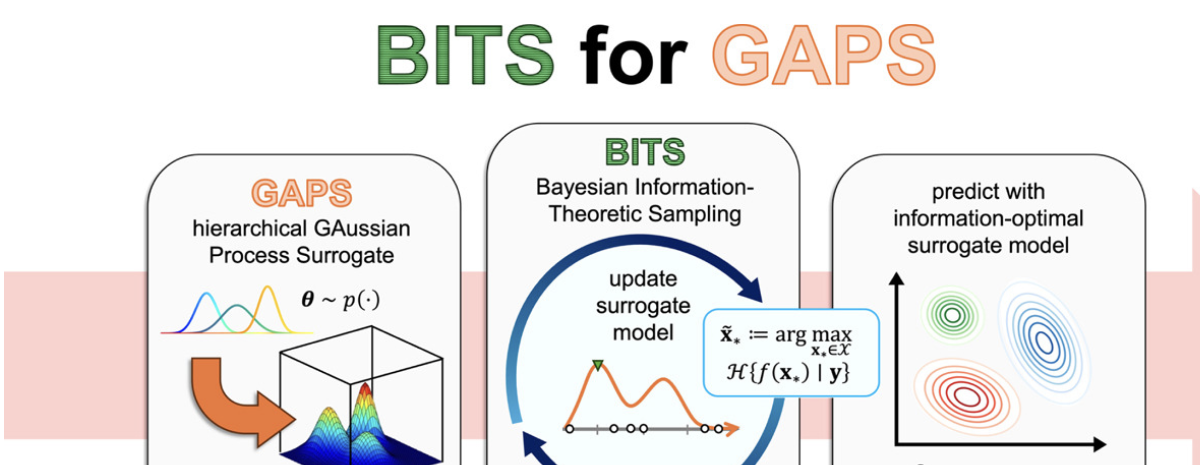
\includegraphics[width=0.58\textwidth]{figures/bits_for_gaps_graphical_abstract}\\[0.15em]
    {\scriptsize K.~D.~Jones and A.~W.~Dowling, \textit{Computers \& Chemical Engineering} \textbf{211} (2026) 109650}
  \end{center}
  \vspace{0.35em}
  \begin{center}
    \slidepoint{After Kyla defended, I turned her well-organized private codebase into a \textbf{public, pip-installable package} using Claude Code.}
  \end{center}
  \vspace{0.8cm plus 1fill}
\end{frame}

\begin{frame}{Task 2: The package conversion recipe}
  \ndlogonote{\scriptsize\href{https://github.com/dowlinglab/claude-for-researchers/blob/main/resources/practices/private_code_to_public_package.md}{\texttt{resources/practices/private\_code\_to\_public\_package.md}}}
  \vfill
  \begin{enumerate}\setlength\itemsep{0.75em}
    \item \textbf{Reproduce the paper} in a clean environment and save trusted outputs.
    \item \textbf{Extract an installable package} while keeping the original results as regression tests.
    \item \textbf{Decompose and generalize} one bounded change at a time.
    \item \textbf{Document and test} a clean installation plus every published figure.
    \item \textbf{Release}: choose a license, then publish to PyPI with GitHub Actions.
  \end{enumerate}
  \vfill
  \begin{center}
    \slidepoint{Every step ends by comparing against the \textbf{published baseline}.}
  \end{center}
  \vspace{1.2cm plus 1fill}
\end{frame}

\begin{frame}{Task 2: Establish a reproducible baseline}
  \ndlogonote{\scriptsize\href{https://github.com/dowlinglab/claude-for-researchers/blob/main/resources/practices/scientific_computing_workflow.md}{\texttt{resources/practices/scientific\_computing\_workflow.md}}}
  \vfill
  \vspace{-0.45cm}
  \begin{enumerate}\setlength\itemsep{0.45em}
    \item \textbf{Find dependency clues} in the paper, report, and codebase.
    \item \textbf{Create a clean Conda environment} from the inferred package versions.
    \item \textbf{Reproduce results systematically}, working from easiest to hardest.
    \item \textbf{Record coverage}: what reproduced, failed, or was not attempted.
    \item \textbf{Freeze the setup}: environment file plus clean-install instructions.
    \item \textbf{Save trusted outputs} as golden regression baselines.
  \end{enumerate}
  \vspace{0.55em}
  \begin{center}\small
    Optional after the baseline is stable: update packages, then repeat the full reproduction.
  \end{center}
  \vfill
\end{frame}

\begin{frame}[fragile]{Task 2: Decompose, generalize, then port}
  \vfill
  \begin{center}
  \begin{tikzpicture}[font=\small]
    \node[nd box, minimum width=3.6cm, minimum height=1.1cm, align=center]
      (a) {\texttt{sampler.py}\\\scriptsize one file, everything};
    \node[nd highlight, minimum width=4.0cm, minimum height=1.1cm, align=center, right=1.2cm of a]
      (b) {\texttt{gp.py}\\\texttt{mixture.py}\\\texttt{acquisition.py}, \ldots};
    \draw[-{Stealth[length=6pt]}, thick] (a) -- (b);
  \end{tikzpicture}
  \end{center}
  \vspace{0.75em}
  \begin{itemize}\setlength\itemsep{0.55em}
    \item Split code so each part can be tested in isolation.
    \item Generalize the verified path before adding a second use case.
    \item Re-run the pinned baseline after every step.
  \end{itemize}
  \vfill
  \begin{center}
    \slidepoint{The package becomes reusable without losing the published case studies that made it credible.}
  \end{center}
  \vspace{1.1cm plus 1fill}
\end{frame}

  \begin{frame}{Best Practices:}
  \vfill
  \begin{columns}[t]
    \begin{column}{0.46\textwidth}
      \textbf{Best practices}
      \begin{itemize}\setlength\itemsep{0.45em}
        \item Put project files in Git.
        \item Record the environment.
        \item Record the run command.
        \item Audit the original result.
        \item Save a baseline.
        \item Test extracted code.
        \item Extend one bounded question.
        \item Write a handoff.
      \end{itemize}
    \end{column}
    \begin{column}{0.49\textwidth}
      \textbf{Research tasks}
      \begin{itemize}\small\setlength\itemsep{0.55em}
        \item \textbf{Task 1: Set up agents and inherit a project}
        \item \textbf{Task 2: Paper code to public package}
        \item Task 3: Idea to literature review, report, or proposal
        \item Task 4: Audit a manuscript
        \item Task 5: Project to manuscript
        \item Task 6: Modernize a course
      \end{itemize}
    \end{column}
  \end{columns}
  \vfill
\end{frame}

  \begin{frame}{Part 1 Activity: A cooled reactor with multiple steady states}
  \vfill
  \begin{columns}[c]
    \begin{column}{0.45\textwidth}
      \centering
      \resizebox{\linewidth}{!}{\begin{tikzpicture}[>=Stealth, thick, color=NDBlue, font=\small]
        \draw[rounded corners=7pt, line width=1.3pt] (0.4,0) rectangle (4.0,3.2);
        \draw[IrishGreen, line width=2pt] (0.15,-0.22) rectangle (4.25,3.42);
        \draw[->, line width=1.2pt] (-1.2,2.5) -- (0.4,2.5);
        \node[align=right, anchor=south east] at (-0.10,2.55) {feed\\$q, C_{Af}, T_f$};
        \draw[->, line width=1.2pt] (4.0,0.7) -- (5.2,0.7);
        \node[align=left, anchor=north west] at (4.35,0.62) {outlet\\$q, C_A, T$};
        \draw[->, IrishGreen, line width=1.2pt] (4.8,2.9) -- (4.25,2.9);
        \node[IrishGreen, align=left, anchor=west] at (4.3,3.3) {coolant $T_c$};
        \node[align=center] at (2.2,1.6) {well mixed\\$A\rightarrow B$};
      \end{tikzpicture}}\\[0.8em]
      {\small $r=k_0 e^{-E/(RT)}C_A$}\par
      {\scriptsize First-order, exothermic teaching model}
    \end{column}
    \begin{column}{0.50\textwidth}
      \begin{itemize}\setlength\itemsep{0.8em}
        \item Feed supplies A; the jacket exchanges heat with coolant.
        \item The notebook solves steady material and energy balances for $C_A$ and $T$.
        \item Sweeps $T_c$ from 285 K to 315 K in increments of 0.5 K.
        \item Tries several solver guesses at each temperature.
      \end{itemize}
    \end{column}
  \end{columns}
  \vfill
  \begin{center}\slidepoint{Question: can one coolant temperature admit several steady states?}\end{center}
  \vfill
\end{frame}

\begin{frame}{Notebook result: three states near $T_c=300$ K}
  \vfill
  \begin{columns}[c]
    \begin{column}{0.65\textwidth}
      \centering
      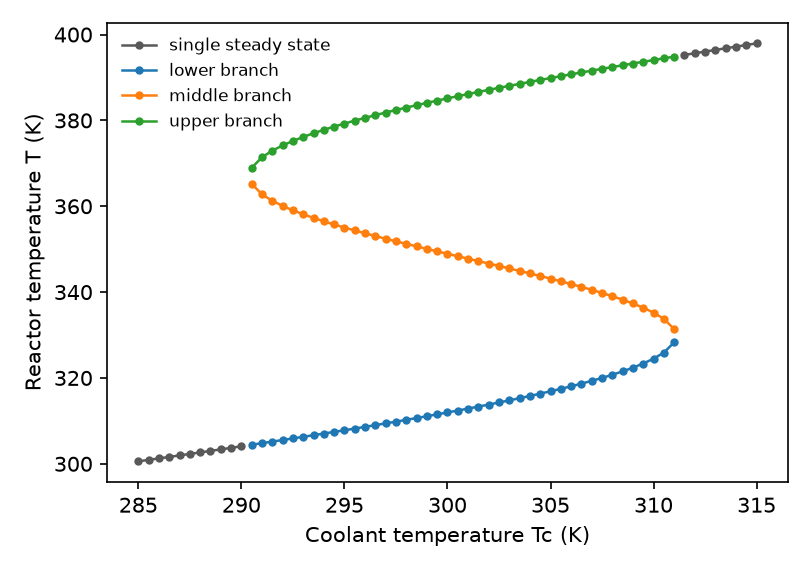
\includegraphics[width=\linewidth,height=5.5cm,keepaspectratio]{figures/cstr_steady_state_locus.png}
    \end{column}
    \begin{column}{0.31\textwidth}
      \begin{itemize}\setlength\itemsep{0.9em}
        \item At $T_c=300$ K, the notebook finds reactor temperatures near 312, 349, and 385 K.
        \item Three states appear from $T_c=290.5$ to 311 K on this grid.
        \item These are steady-state solutions, not stability results.
      \end{itemize}
    \end{column}
  \end{columns}
  \vfill
  \ndlogonote{\scriptsize Original notebook output; teaching parameters; 0.5 K sweep resolution}
\end{frame}

  \begin{frame}{Activity 1: put an inherited notebook in Git}
  \vfill
  \begin{columns}[c]
    \begin{column}{0.42\textwidth}
      \textbf{Start with the reactor notebook.}\\[0.8em]
      {\small Put its inputs, environment, changes, and results in Git so someone else can rerun and extend the work.}\\[1em]
      {\small The ZIP contains the notebook and parameter file. The handout walks through the steps.}\\[1em]
      {\small\href{https://raw.githubusercontent.com/dowlinglab/claude-for-researchers/main/resources/workshops/cstr/workshop1_notebook.zip}{\textbf{Download the notebook ZIP}}}
    \end{column}
    \begin{column}{0.54\textwidth}
      \centering
      \fbox{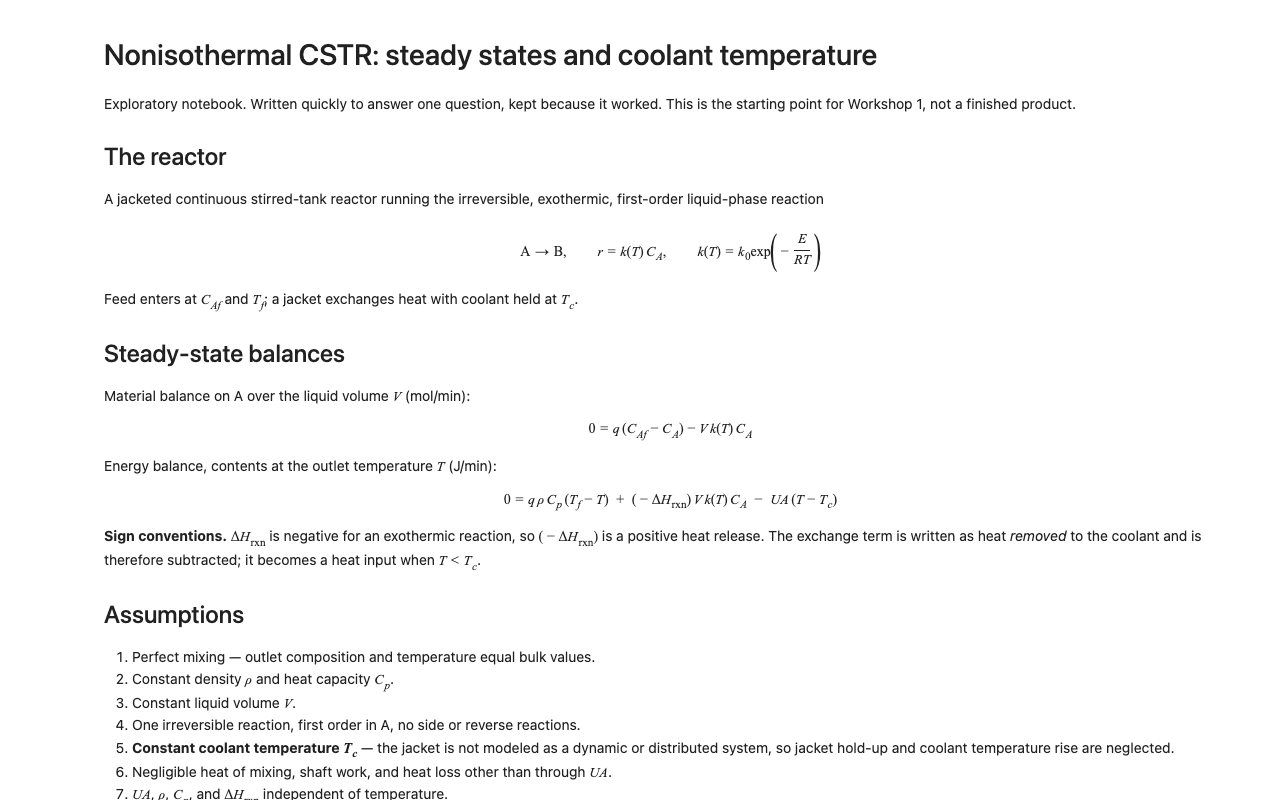
\includegraphics[width=0.94\linewidth]{figures/cstr_notebook_preview.png}}\\[0.3em]
      {\scriptsize The inherited CSTR notebook}
    \end{column}
  \end{columns}
  \vfill
  \ndlogonote{\scriptsize Hands-on: 45 minutes; regroup: 15 minutes}
\end{frame}

\begin{frame}{First, preserve what the inherited notebook does}
  \vfill
  \begin{enumerate}\setlength\itemsep{1em}
    \item \textbf{Create a private repository}
      \begin{itemize}\small
        \item If needed, create a GitHub account and install GitHub Desktop.
        \item Download the ZIP file (notebook and YAML parameter data).
        \item Initialize Git.
        \item Commit the original files.
        \item Connect your private GitHub repository.
      \end{itemize}
    \item \textbf{Run and audit the notebook}
      \begin{itemize}\small
        \item Build the Conda environment.
        \item Run all notebook cells in a fresh kernel.
        \item Check the equations and input parameters.
        \item Check solver convergence and residuals.
        \item Check the saved CSV and figure.
        \item Commit the baseline before refactoring.
      \end{itemize}
  \end{enumerate}
  \vfill
  \ndlogonote{\scriptsize See the Part 1 handout for commands and full instructions}
\end{frame}

\begin{frame}{Then extract, test, and extend one question}
  \vfill
  \begin{enumerate}\setlength\itemsep{1em}
    \setcounter{enumi}{2}
    \item \textbf{Extract and verify functions}
      \begin{itemize}\small
        \item Extract the model equations into a Python file.
        \item Extract the steady-state solver.
        \item Extract the operating-condition sweep.
        \item Extract the plotting code.
        \item Add NumPy-style docstrings.
        \item Test against the saved baseline.
      \end{itemize}
    \item \textbf{Explore one new question}
      \begin{itemize}\small
        \item Choose one of the four extension questions.
        \item Save a runnable command.
        \item Save its result.
        \item Add a test.
        \item Write a short interpretation.
      \end{itemize}
  \end{enumerate}
  \vfill
\end{frame}

  \begin{frame}{Regroup 1: how far did you get?}
  \vfill
  \begin{columns}[c]
    \begin{column}{0.52\textwidth}
      \begin{enumerate}\setlength\itemsep{0.45em}
        \item Found the repository root
        \item Made a first commit
        \item Connected to GitHub
        \item Kept going: run, audit, extend
      \end{enumerate}
    \end{column}
    \begin{column}{0.42\textwidth}
      \slidepoint{What did you ask Claude that helped?}
      \par\vspace{1.5em}\noindent
      \slidepoint{What surprised you?}
      \par\vspace{1.5em}\noindent
      \slidepoint{What will you do next in your research?}
    \end{column}
  \end{columns}
  \vfill
  \ndlogonote{\scriptsize Regroup: 15 minutes; participants share first}
\end{frame}

  \partoneregroup
  \begin{frame}{Part 1 Recap}
  \vfill
  \begin{columns}[c]
    \begin{column}{0.54\textwidth}
      \centering
      \large
      \begin{tabular}{@{}l@{\hspace{0.5cm}}l@{}}
        \textbf{Part 1} & \color{NDGold!80!black}\textbf{Prologue:} \textbf{\color{NDBlue}Tinker} \\[0.8em]
        & \color{NDGold!80!black}\textbf{Act I:} \textbf{\color{NDBlue}Understand} \\[0.8em]
        & \color{NDGold!80!black}\textbf{Act II:} \textbf{\color{NDBlue}Build} \\[1.1em]
        \textbf{Part 2} & \color{NDGold!80!black}\textbf{Act III:} \textbf{\color{NDBlue}Challenge} \\[0.8em]
        & \color{NDGold!80!black}\textbf{Epilogue:} \textbf{\color{NDBlue}Trust}
      \end{tabular}
    \end{column}
    \begin{column}{0.42\textwidth}
      \textbf{Takeaways}
      \begin{itemize}\setlength\itemsep{0.7em}
        \item Work in a Git repository.
        \item Give agents project context.
        \item Run and audit before refactoring.
        \item Ask, inspect, verify, iterate.
      \end{itemize}
    \end{column}
  \end{columns}
  \vfill
\end{frame}

\fi

\ifnum\seminarpart=1\else
  \sessiontitle{Part 2}{Advanced features}{12 October 2026}
  \begin{frame}{Part 1 Recap}
  \vfill
  \begin{columns}[c]
    \begin{column}{0.54\textwidth}
      \centering
      \large
      \begin{tabular}{@{}l@{\hspace{0.5cm}}l@{}}
        \textbf{Part 1} & \color{NDGold!80!black}\textbf{Prologue:} \textbf{\color{NDBlue}Tinker} \\[0.8em]
        & \color{NDGold!80!black}\textbf{Act I:} \textbf{\color{NDBlue}Understand} \\[0.8em]
        & \color{NDGold!80!black}\textbf{Act II:} \textbf{\color{NDBlue}Build} \\[1.1em]
        \textbf{Part 2} & \color{NDGold!80!black}\textbf{Act III:} \textbf{\color{NDBlue}Challenge} \\[0.8em]
        & \color{NDGold!80!black}\textbf{Epilogue:} \textbf{\color{NDBlue}Trust}
      \end{tabular}
    \end{column}
    \begin{column}{0.42\textwidth}
      \textbf{Takeaways}
      \begin{itemize}\setlength\itemsep{0.7em}
        \item Work in a Git repository.
        \item Give agents project context.
        \item Run and audit before refactoring.
        \item Ask, inspect, verify, iterate.
      \end{itemize}
    \end{column}
  \end{columns}
  \vfill
\end{frame}

  \begin{frame}{Part 1 used Git and GitHub. What was happening?}
  \vfill
  \begin{center}
    \slidepoint{You already \textbf{used} Git and GitHub.}\\[1.3em]
    \slidepoint{Let's review the concepts in \textbf{five illustrations}.}
  \end{center}
  \vfill
\end{frame}

  \begin{frame}{Git keeps history locally; GitHub hosts a copy}
  \vfill
  \begin{center}
    \resizebox{0.94\linewidth}{!}{% Figure 1: local folder -> local Git repository -> GitHub remote.
% Uses the nd box / nd highlight styles from main.tex.
\begin{tikzpicture}[font=\small\sffamily, >=Stealth]
  \node[nd box, minimum width=4.4cm, minimum height=2.3cm] (folder) at (0,0)
    {\textbf{Project folder}\\[3pt]{\footnotesize the files you edit:}\\{\footnotesize code, notebooks, text}};
  \node[nd highlight, minimum width=4.8cm, minimum height=2.3cm] (repo) at (6.6,0)
    {\textbf{Local Git repository}\\[3pt]{\footnotesize the history of your project,}\\{\footnotesize kept on your computer}};
  \node[nd box, minimum width=4.4cm, minimum height=2.3cm] (gh) at (13.2,0)
    {\textbf{GitHub}\\[3pt]{\footnotesize a copy of the repository}\\{\footnotesize on the web}};
  \draw[->, very thick, NDBlue] ([yshift=0.25cm]folder.east) -- node[above, font=\footnotesize\bfseries] {commit} ([yshift=0.25cm]repo.west);
  \draw[->, very thick, NDBlue] ([yshift=0.25cm]repo.east) -- node[above, font=\footnotesize\bfseries] {push} ([yshift=0.25cm]gh.west);
  \draw[<-, very thick, NDBlue] ([yshift=-0.25cm]repo.east) -- node[below, font=\footnotesize\bfseries] {pull} ([yshift=-0.25cm]gh.west);
  \draw[decorate, decoration={brace, amplitude=7pt, mirror}, NDBlue, thick] (-2.2,-1.5) -- node[below=9pt, font=\footnotesize] {on your computer} (9.0,-1.5);
  \draw[decorate, decoration={brace, amplitude=7pt, mirror}, NDBlue, thick] (11.0,-1.5) -- node[below=9pt, font=\footnotesize] {on the web} (15.4,-1.5);
\end{tikzpicture}
}
  \end{center}
  \vspace{0.9em}
  \begin{center}\small
    \textbf{Git} is the version-control tool. \textbf{GitHub} hosts a copy and helps people collaborate.
  \end{center}
  \vspace{1.6cm plus 1fill}
\end{frame}
\begin{frame}{A commit is a labeled checkpoint, not a save}
  \vfill
  \begin{center}
    \resizebox{0.94\linewidth}{!}{% Figure 2: commit history as a series of checkpoints, with what is on GitHub.
\begin{tikzpicture}[font=\small\sffamily, >=Stealth]
  \foreach \x/\msg/\hash [count=\i] in {0/{Import\\inherited notebook}/a3f9c1e, 3.9/{Record the\\environment}/7b21d04, 7.8/{Save baseline\\results}/e90c5a2, 11.7/{Extract tested\\functions}/4d18b7f} {
    \node[circle, draw=NDGold, line width=1.2pt, fill=white, minimum size=0.9cm, inner sep=0pt] (c\i) at (\x,0) {};
    \node[text=NDBlue, align=center, text width=3.4cm] at (\x,1.25) {\textbf{\msg}};
    \node[text=NDBlue, font=\ttfamily\footnotesize] at (\x,-0.95) {\hash};
  }
  \foreach \a/\b in {1/2, 2/3, 3/4} { \draw[->, very thick, NDBlue] (c\a) -- (c\b); }
  \node[circle, draw=IrishGreen, line width=2pt, fill=white, minimum size=0.9cm, inner sep=0pt] at (11.7,0) {};
  \draw[decorate, decoration={brace, amplitude=6pt, mirror}, NDBlue, thick] (-0.6,-1.55) -- node[below=8pt, font=\footnotesize] {also on GitHub (pushed)} (8.4,-1.55);
  \node[text=NDBlue, font=\footnotesize, align=center] at (11.7,-2.4) {newest commit,\\not pushed yet};
  \draw[->, NDBlue] (14.1,0) -- node[above, font=\footnotesize] {time} (15.4,0);
\end{tikzpicture}
}
  \end{center}
  \vspace{0.9em}
  \begin{center}\small
    Commit when the project is in a state you would want to return to, with a message that says why.
  \end{center}
  \vspace{1.6cm plus 1fill}
\end{frame}
\begin{frame}[fragile]{The repository root, and what Git ignores}
  \vfill
  \begin{columns}[c]
    \begin{column}{0.50\textwidth}
      \begin{lstlisting}[basicstyle=\ttfamily\footnotesize]
research-project/  <- root
  .git/            <- history
  .gitignore       <- skip list
  code/
  notebooks/
  results/         <- ignored
      \end{lstlisting}
    \end{column}
    \begin{column}{0.46\textwidth}
      \begin{itemize}\setlength\itemsep{0.8em}
        \item The \textbf{root} is the folder that contains \texttt{.git}. Git tracks the project relative to it.
        \item \texttt{.gitignore} lists files Git should skip: caches, environments, and regenerable output.
      \end{itemize}
    \end{column}
  \end{columns}
  \vspace{0.9em}
  \begin{center}\small
    Ask Claude: ``What should this project ignore, and why?''
  \end{center}
  \vspace{1.4cm plus 1fill}
\end{frame}
\begin{frame}{Never nest one Git repository inside another}
  \vfill
  \begin{center}
    \resizebox{0.94\linewidth}{!}{% Figure 4: a good repository layout beside the nested-repository problem.
\begin{tikzpicture}[font=\small\sffamily, >=Stealth]
  \node[nd highlight, anchor=north west, inner sep=8pt, align=left, text width=6.2cm] (good) at (0,0) {%
    \good{\textbf{One repository}}\\[4pt]
    {\ttfamily\footnotesize
    research-project/\hfill\textcolor{IrishGreen}{$\leftarrow$ Git repo}\\
    \hspace*{1em}code/\\
    \hspace*{1em}notebooks/\\
    \hspace*{1em}data-small/\\
    \hspace*{1em}README.md\\
    \hspace*{1em}.gitignore}};
  \node[nd box, draw=OkVermillion, anchor=north west, inner sep=8pt, align=left, text width=7.2cm] (bad) at (7.2,0) {%
    \bad{\textbf{A repository inside another}}\\[4pt]
    {\ttfamily\footnotesize
    research-project/\hfill\textcolor{OkVermillion}{$\leftarrow$ Git repo}\\
    \hspace*{1em}analysis/\\
    \hspace*{2em}another-project/\hfill\textcolor{OkVermillion}{$\leftarrow$ another Git repo}\\
    \hspace*{1em}README.md\\
    \hspace*{1em}.gitignore}};
\end{tikzpicture}
}
  \end{center}
  \vspace{0.9em}
  \begin{center}\small
    The outer repository does not track the inner one's files, and tools can disagree about which history applies.\\[0.5em]
    You can use submodules for certain cases (advanced users).
  \end{center}
  \vspace{1.2cm plus 1fill}
\end{frame}
\begin{frame}{Track text in GitHub; keep big files elsewhere}
  \vfill
  \begin{center}
    \resizebox{0.86\linewidth}{!}{% Figure 3: which kinds of artifacts tend to belong in GitHub and which in other storage.
\begin{tikzpicture}[font=\small\sffamily, >=Stealth]
  \node[nd highlight, text width=6.2cm, inner sep=8pt, align=left, minimum height=4.1cm, anchor=north west] (git) at (0,0)
    {\centering\textbf{GitHub (Git repository)}\\[4pt]
     \footnotesize\raggedright
     source code and scripts\\ text, Markdown, LaTeX\\ configuration files\\ documentation and notes\\ small data files\\ notebooks (with caveats)};
  \node[nd box, text width=6.9cm, inner sep=8pt, align=left, minimum height=4.1cm, anchor=north west] (store) at (7.4,0)
    {\centering\textbf{Cloud or institutional storage}\\[4pt]
     \footnotesize\raggedright
     large raw datasets\\ PDFs, images, and slide decks\\ instrument output\\ large binary files\\ archives you rarely change\\[3pt]
     {\scriptsize e.g. Google Drive, OneDrive, shared lab storage, or a research data repository}};
  \node[nd box, minimum width=14.3cm, anchor=north west, inner sep=6pt] at (0,-4.5)
    {\footnotesize One project can span both. A README or data note says where each large file lives and how to get it.};
\end{tikzpicture}
}
  \end{center}
  \vspace{0.6em}
  \begin{center}\small
    My working limit is about \textbf{10 MB} per Git file. GitHub blocks ordinary files over 100 MiB.
  \end{center}
  \vspace{1.6cm plus 1fill}
\end{frame}

  \stagedivider{3}{Act II: Build}{Create reusable software and literature-grounded documents}

\taskdivider{3}

\begin{frame}{Task 3: Idea to a literature review, report, or proposal}
  \ndlogonote{\scriptsize\href{https://github.com/dowlinglab/claude-for-researchers/blob/main/resources/practices/technical_writing.md}{\texttt{resources/practices/technical\_writing.md}}}
  \vfill
  \begin{columns}[t]
    \begin{column}{0.46\textwidth}
      \textbf{What is \LaTeX?}
      \begin{itemize}\small\setlength\itemsep{0.4em}
        \item a plain-text document source
        \item separates content from layout
        \item compiles to a PDF
        \item built for equations, references, and cross-references
      \end{itemize}
    \end{column}
    \begin{column}{0.48\textwidth}
      \textbf{Why agents work well with it}
      \begin{itemize}\small\setlength\itemsep{0.4em}
        \item the source is searchable text
        \item sections and figures are separate files
        \item every edit produces a readable diff
        \item the compiled PDF is a visual check
      \end{itemize}
    \end{column}
  \end{columns}
  \vspace{1.0em}
  \begin{center}
    \slidepoint{\textbf{Plain text} (e.g., \LaTeX, not MS Word) allows an agent and Git to effectively work with your document (manuscript, proposal, report).}
  \end{center}
  \vspace{1.1cm plus 1fill}
\end{frame}

\begin{frame}{Overleaf and local edits meet through GitHub}
  \ndlogonote{\scriptsize\href{https://docs.overleaf.com/integrations-and-add-ons/git-integration-and-github-synchronization/github-synchronization}{Overleaf: GitHub synchronization (documentation + screenshot)}\quad\href{https://github.com/dowlinglab/claude-for-researchers/blob/main/resources/practices/latex_overleaf_workflow.md}{Companion workflow}}
  \vfill
  \begin{columns}[c]
    \begin{column}{0.46\textwidth}
      \centering
      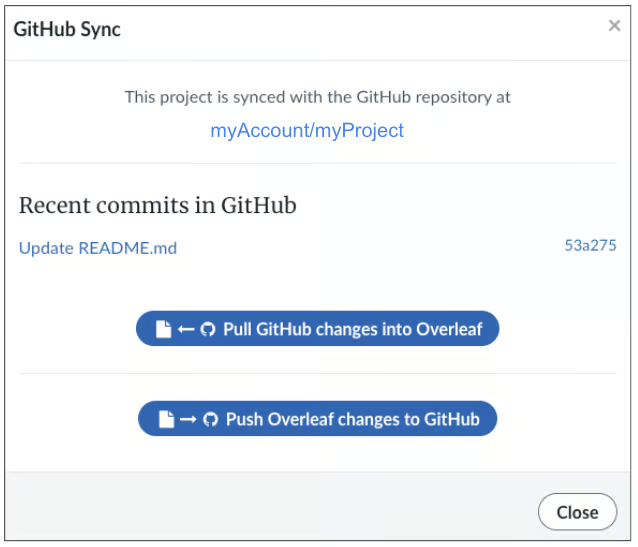
\includegraphics[width=\linewidth,height=4.9cm,keepaspectratio]{figures/overleaf_github_sync.png}
    \end{column}
    \begin{column}{0.49\textwidth}
      \begin{enumerate}\small\setlength\itemsep{0.7em}
        \item Sync Overleaf edits to GitHub; pull locally.
        \item Revise on a \textbf{feature branch}.
        \item Incorporate collaborators' latest changes; review and merge.
        \item Pull the merged version into Overleaf.
      \end{enumerate}
      \vspace{0.5em}
      \small Synchronization is \textbf{explicit}, not automatic. Coordinate with coauthors.
    \end{column}
  \end{columns}
  \vspace{0.8cm plus 1fill}
\end{frame}

\begin{frame}{Three repositories keep development, writing, and release separate}
  \ndlogonote{\scriptsize\href{https://github.com/dowlinglab/claude-for-researchers/blob/main/resources/practices/latex_overleaf_workflow.md}{\texttt{resources/practices/latex\_overleaf\_workflow.md}}}
  \vfill
  \begin{center}\small
  \renewcommand{\arraystretch}{1.22}
  \begin{tabular}{@{}>{\raggedright\arraybackslash}p{3.1cm}>{\raggedright\arraybackslash}p{5.1cm}>{\raggedright\arraybackslash}p{4.3cm}@{}}
    \toprule
    \textbf{Repository} & \textbf{What belongs there} & \textbf{History} \\
    \midrule
    Private code & data, experiments, analysis & rich history; my projects: 10--500 MB \\
    Private writing & \LaTeX{}, bibliography, selected figures & compact history; sync recommendation: $<100$ MB \\
    Public release & package and paper reproduction & near-final history for readers \\
    \bottomrule
  \end{tabular}
  \end{center}
  \vspace{0.7em}
  \begin{itemize}\small\setlength\itemsep{0.4em}
    \item Keep individual Git files below about \textbf{10 MB}.
    \item Put large PDF collections on a shared drive, not in Git.
    \item Keep the summaries and \texttt{ref.bib} in Git.
  \end{itemize}
  \vspace{1.0cm plus 1fill}
\end{frame}

\begin{frame}{Task 3, step 1: Search, read, and search again}
  \ndlogonote{\scriptsize\href{https://github.com/dowlinglab/claude-for-researchers/blob/main/resources/practices/literature_review.md}{\texttt{resources/practices/literature\_review.md}}}
  \vfill
  \begin{enumerate}\setlength\itemsep{0.8em}
    \item \textbf{Frame the question with a chatbot}
      \begin{itemize}\small
        \item develop terminology, synonyms, and adjacent disciplines
        \item turn the idea into several targeted search strings
      \end{itemize}
    \item \textbf{Search Google Scholar and disciplinary databases}
      \begin{itemize}\small
        \item follow review papers, citation trails, and competing terminology
        \item download only papers you can identify and inspect
      \end{itemize}
    \item \textbf{Repeat after each processed batch}
      \begin{itemize}\small
        \item ask the agent which gaps, authors, and references should drive the next search
      \end{itemize}
  \end{enumerate}
  \vspace{1.0cm plus 1fill}
\end{frame}

\begin{frame}{Task 3, step 2: Build a literature corpus an agent can use}
  \ndlogonote{\scriptsize\href{https://github.com/dowlinglab/claude-for-researchers/blob/main/resources/prompts/literature_workflow.md}{\texttt{resources/prompts/literature\_workflow.md}}}
  \vfill
  \begin{enumerate}\setlength\itemsep{0.8em}
    \item \textbf{Process the PDFs in small topical batches}
      \begin{itemize}\small
        \item checkpoint after each batch
        \item propose consistent filenames; flag likely duplicates without deleting
      \end{itemize}
    \item \textbf{Maintain \texttt{ref.bib} as you go}
      \begin{itemize}\small
        \item verified metadata and DOI information, one entry per paper
      \end{itemize}
    \item \textbf{Summarize every paper in \texttt{literature.md}}
      \begin{itemize}\small
        \item contribution, evidence, relevance, and what it cannot support
        \item keep the PDFs in a reference manager; keep the text artifacts in Git
      \end{itemize}
  \end{enumerate}
  \vspace{0.6em}
  \begin{center}
    \slidepoint{The durable product is the \textbf{verified map of the literature}.}
  \end{center}
  \vspace{0.6cm plus 1fill}
\end{frame}

\begin{frame}{Task 3, step 3: Edit the document against the curated corpus}
  \ndlogonote{\scriptsize\href{https://github.com/dowlinglab/claude-for-researchers/blob/main/resources/practices/grant_proposal_writing.md}{\texttt{resources/practices/grant\_proposal\_writing.md}}}
  \vfill
  \begin{enumerate}\setlength\itemsep{0.8em}
    \item \textbf{Start from the question and \texttt{literature.md}}
      \begin{itemize}\small
        \item build a claim-and-evidence outline before writing prose
      \end{itemize}
    \item \textbf{Draft one section at a time}
      \begin{itemize}\small
        \item ask what evidence supports each paragraph before polishing it
        \item preserve uncertainty and conflicting evidence as part of the argument
      \end{itemize}
    \item \textbf{Check every claim against the source PDFs}
      \begin{itemize}\small
        \item edit against the local corpus, not an agent's memory
      \end{itemize}
  \end{enumerate}
  \vspace{1.0cm plus 1fill}
\end{frame}

\begin{frame}{Review the source diff and the manuscript diff}
  \ndlogonote{\scriptsize\href{https://github.com/dowlinglab/claude-for-researchers/tree/main/resources/examples/manuscript_revision}{Reproduce the example}\quad\href{https://docs.github.com/en/desktop/making-changes-in-a-branch/committing-and-reviewing-changes-to-your-project-in-github-desktop}{Screenshot: GitHub Docs}}
  \vfill
  \begin{columns}[c]
    \begin{column}{0.48\textwidth}
      \centering\small\textbf{GitHub Desktop: file changes}\\[0.5em]
      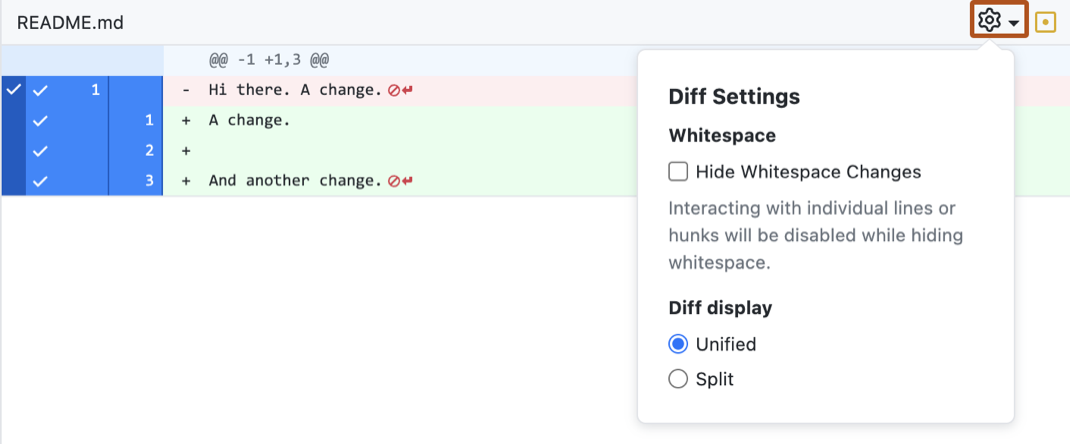
\includegraphics[width=\linewidth]{figures/github_desktop_diff.png}
    \end{column}
    \begin{column}{0.48\textwidth}
      \centering\small\textbf{\texttt{latexdiff}: manuscript changes}\\[0.5em]
      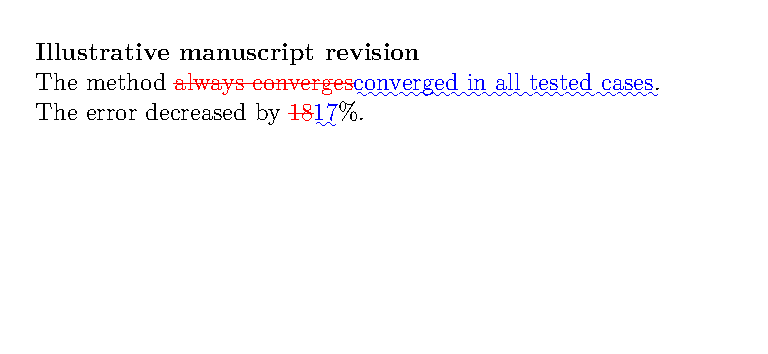
\includegraphics[width=\linewidth]{figures/manuscript_diff.pdf}
    \end{column}
  \end{columns}
  \vspace{0.8em}
  \begin{center}\small
    Ask the agent to generate and compile \texttt{latexdiff}.\\[0.35em]
    \textbf{You review the changed claims} before merging and syncing.
  \end{center}
  \vspace{0.8cm plus 1fill}
\end{frame}

  \stagedivider{4}{Act III: Challenge}{Use the accumulated evidence to test and extend the work}

\taskdivider{4}

\begin{frame}{Task 4: Audit a manuscript before submission}
  \ndlogonote{\scriptsize\href{https://github.com/dowlinglab/claude-for-researchers/blob/main/resources/prompts/manuscript_audit.md}{\texttt{resources/prompts/manuscript\_audit.md}}}
  \vspace{0.15em}
  {\normalsize
    \textbf{Prerequisites}\par
    \begin{itemize}\normalsize\setlength\itemsep{0.05em}
      \item Manuscript and analysis under version control
      \item A working computational environment
      \item The Task 3 literature corpus available to the agent
    \end{itemize}
  }
  \vspace{0.3em}
  {\large\textbf{Audit Goals}\par}
  \begin{enumerate}\large\setlength\itemsep{0.25em}
    \item Do the methods match what the code did?
    \item Can every reported number be recomputed and traced to a results artifact?
    \item Do figure labels, captions, and prose agree with the data?
    \item Do literature claims match the source papers?
    \item Does the manuscript meet the journal's current author guidelines?
  \end{enumerate}
  \vspace{1.0cm plus 1fill}
\end{frame}

\begin{frame}{Task 4: Trace each claim to evidence}
  \ndlogonote{\scriptsize\href{https://github.com/dowlinglab/claude-for-researchers/blob/main/resources/templates/results_manifest.md}{\texttt{resources/templates/results\_manifest.md}}}
  \vfill
  \begin{center}
  \renewcommand{\arraystretch}{1.25}
  \begin{tabular}{@{}p{5.1cm}p{2.5cm}p{2.7cm}l@{}}
    \toprule
    \textbf{Manuscript claim} & \textbf{Location} & \textbf{Source} & \textbf{Status} \\
    \midrule
    Costs decrease by 17\% & Results \S4.2 & \texttt{cost.csv} & \good{Verified} \\
    Reaction proceeds in 3 steps & Methods \S2.1 & \texttt{mechanism.py} & \bad{Mismatch (4)} \\
    Yield approximately doubles & Abstract & unknown & \unknown{Cannot verify} \\
    \bottomrule
  \end{tabular}
  \end{center}
  \vspace{0.65em}
  \begin{columns}[t]
    \begin{column}{0.48\textwidth}
      \small\textbf{Arithmetic}\par Recompute from the underlying values rather than rereading the displayed number.
    \end{column}
    \begin{column}{0.48\textwidth}
      \small\textbf{Traceability}\par Search the repository for the claim and name the exact file, or report that no source was found.
    \end{column}
  \end{columns}
  \vfill
  \begin{center}
    \slidepoint{\textbf{Cannot verify} identifies a real \textbf{provenance gap}.}
  \end{center}
  \vspace{1.0cm plus 1fill}
\end{frame}

\begin{frame}{The DOI checker has two verification modes}
  \ndlogonote{\scriptsize\href{https://github.com/dowlinglab/claude-for-researchers/tree/main/resources/scripts/doi_checker}{\texttt{resources/scripts/doi\_checker/}}}
  \vfill
  \begin{center}
  \begin{tikzpicture}[font=\small,
      doi mode/.style={nd box, text width=4.0cm,
        minimum height=1.5cm, inner sep=0.1cm, align=center}]
    \node[nd box, text width=2.2cm,
      minimum height=1.2cm, align=center] (a) at (0,0)
      {Versioned\\\texttt{ref.bib}};
    \node[doi mode] (b) at (4.7,1.05)
      {\textbf{Existing DOI}\\{\scriptsize Crossref: title + first author}};
    \node[doi mode] (c) at (4.7,-1.05)
      {\textbf{Missing DOI}\\{\scriptsize Search Crossref and\\rank candidate matches}};
    \node[nd highlight, text width=3.4cm,
      minimum height=1.5cm, align=center] (d) at (10,0)
      {Reviewable report\\{\scriptsize match, check, mismatch,\\unresolved; candidates}};
    \coordinate (split) at (1.9,0);
    \coordinate (merge) at (7.55,0);
    \draw[thick] (a.east) -- (split);
    \draw[-{Stealth[length=6pt]}, thick] (split) |- (b.west);
    \draw[-{Stealth[length=6pt]}, thick] (split) |- (c.west);
    \draw[thick] (b.east) -| (merge);
    \draw[thick] (c.east) -| (merge);
    \draw[-{Stealth[length=6pt]}, thick] (merge) -- (d.west);
  \end{tikzpicture}
  \end{center}
  \vspace{0.7em}
  \begin{center}\small
    The tool reports only. It never edits the bibliography, and it cannot decide whether a paper supports the sentence that cites it.
  \end{center}
  \vspace{1.15cm plus 1fill}
\end{frame}

\taskdivider{5}

\begin{frame}{Task 5: Draft a manuscript from the previous tasks}
  \ndlogonote{\scriptsize\href{https://github.com/dowlinglab/claude-for-researchers/blob/main/resources/practices/technical_writing.md}{\texttt{resources/practices/technical\_writing.md}}}
  \vspace{0.15cm}
  \begin{center}
  \begin{tikzpicture}[font=\small, node distance=0.30cm,
      task box/.style={nd box, minimum height=0.68cm,
        inner xsep=0.18cm, align=center}]
    \node[task box]
      (a) {\textbf{Task 1}: versioned workspace, environment, instructions, reproducible baseline};
    \node[task box, below=of a]
      (b) {\textbf{Task 2}: trustworthy software, figures, and results};
    \node[task box, below=of b]
      (c) {\textbf{Task 3}: curated literature, bibliography, and claim-evidence outline};
    \node[task box, below=of c]
      (d) {\textbf{Task 4}: audit questions and traceability checks};
    \node[font=\small, inner sep=0pt] at ($(a.south)!0.5!(b.north)$) {$+$};
    \node[font=\small, inner sep=0pt] at ($(b.south)!0.5!(c.north)$) {$+$};
    \node[font=\small, inner sep=0pt] at ($(c.south)!0.5!(d.north)$) {$+$};
    \node[task box, draw=IrishGreen, minimum height=0.76cm, below=0.38cm of d]
      (e) {\textbf{Task 5}: a manuscript with evidence attached};
    \draw[-{Stealth[length=7pt]}, thick] (d.south) -- (e.north);
  \end{tikzpicture}
  \end{center}
  \vspace{0.25em}
  \begin{center}
    \slidepoint{Drafting becomes an \textbf{integration task}, not a blank-page task.}
  \end{center}
  \vspace{0.7cm plus 1fill}
\end{frame}

\begin{frame}{Task 5: Figures first, then outline, sections, and revision}
  \ndlogonote{\scriptsize\href{https://github.com/dowlinglab/claude-for-researchers/blob/main/resources/practices/scientific_figures_tables.md}{\texttt{resources/practices/scientific\_figures\_tables.md}}\quad\href{https://github.com/dowlinglab/claude-for-researchers/blob/main/resources/practices/writing_style_guide.md}{\texttt{writing\_style\_guide.md}}}
  \vspace{0.02cm}
  \begin{columns}[c]
    \begin{column}{0.44\textwidth}
      \centering
      \begin{tikzpicture}[font=\small, node distance=0.30cm,
          flowstep/.style={nd box, minimum width=4.3cm, minimum height=0.78cm, align=center}]
        \node[flowstep] (a) {Develop the key figures};
        \node[flowstep, below=of a] (b) {Outline claims around figures};
        \node[flowstep, below=of b] (c) {Draft one section at a time};
        \node[flowstep, below=of c] (d) {Edit against corpus and style guide};
        \node[flowstep, draw=IrishGreen, below=of d] (e) {Audit, render, and revise};
        \draw[-{Stealth[length=6pt]}, thick] (a) -- (b);
        \draw[-{Stealth[length=6pt]}, thick] (b) -- (c);
        \draw[-{Stealth[length=6pt]}, thick] (c) -- (d);
        \draw[-{Stealth[length=6pt]}, thick] (d) -- (e);
      \end{tikzpicture}
    \end{column}
    \begin{column}{0.50\textwidth}
      \textbf{The agent can help\ldots}
      \begin{itemize}\setlength\itemsep{0.40em}
        \item reproduce computational experiments
        \item create and edit figures
        \item organize the argument
        \item draft sections
        \item check the literature corpus
        \item complete a final manuscript audit
      \end{itemize}
    \end{column}
  \end{columns}
  \vspace{0.9em}
  \begin{center}
    \slidepoint{The researcher made every \textbf{scientific and editorial decision}.}
  \end{center}
  \vspace{0.65cm plus 1fill}
\end{frame}

\taskdivider{6}

\begin{frame}{Task 6: Modernize my graduate elective}
  \ndlogonote{\scriptsize retired: \href{https://ndcbe.github.io/CBE60499/}{\texttt{ndcbe.github.io/CBE60499/}}\\current: \href{https://ndcbe.github.io/optimization/}{\texttt{ndcbe.github.io/optimization/}}}
  \vfill
  \begin{center}
  \resizebox{0.96\textwidth}{!}{%
  \begin{tikzpicture}[
    font=\small,
    node distance=0.32cm,
    offering/.style={nd box, minimum width=2.4cm, minimum height=2.6cm, text width=2.1cm, align=center}
  ]
    \node[offering]
      (y2018) {\textbf{Fall 2018}\\[0.3em]handwritten notes\\[0.22em]Jupyter notebooks};
    \node[offering, right=of y2018]
      (y2021) {\textbf{Spring 2021}\\[0.3em]\texttt{nbpages} website\\[0.22em]applications first};
    \node[offering, right=of y2021]
      (y2023) {\textbf{Spring 2023}\\[0.3em]\texttt{JupyterBook} website};
    \node[offering, right=of y2023]
      (y2024) {\textbf{Fall 2024}\\[0.3em]iterative refinement};
    \node[offering, right=of y2024]
      (y2026) {\textbf{Fall 2026}\\[0.3em]coursepack\\[0.22em]AI-forward redesign};
    \draw[-{Stealth[length=6pt]}, thick] (y2018) -- (y2021);
    \draw[-{Stealth[length=6pt]}, thick] (y2021) -- (y2023);
    \draw[-{Stealth[length=6pt]}, thick] (y2023) -- (y2024);
    \draw[-{Stealth[length=6pt]}, thick] (y2024) -- (y2026);
  \end{tikzpicture}}
  \end{center}
  \vspace{0.8em}
  \begin{center}
    {\small Fall 2018: theory + algorithms $\longrightarrow$ applications}\\[0.45em]
    {\small\color{NDBlue}Since Spring 2021: applications $\longrightarrow$ theory + algorithms}
  \end{center}
  \vspace{1.65cm plus 1fill}
\end{frame}

\begin{frame}{Four Goals... Starting One Week Before the First Lecture}
  \vfill
  \begin{columns}[c]
    \begin{column}{0.54\textwidth}
      \begin{enumerate}\footnotesize\setlength\itemsep{0.45em}
        \item \textbf{Deferred maintenance}
          \begin{itemize}\footnotesize\item update the website and computational examples\end{itemize}
        \item \textbf{Coursepack with strategic gaps}
          \begin{itemize}\footnotesize\item reduce math copying; create time for active learning\end{itemize}
        \item \textbf{AI-forward assessment}
          \begin{itemize}\footnotesize\item explicit AI policy and completion-based homework grading
            \item assessment analytics and an AI-forward project\end{itemize}
        \item \textbf{More in-class exams}
          \begin{itemize}\footnotesize\item open coursepack; assess individual understanding\end{itemize}
      \end{enumerate}
    \end{column}
    \begin{column}{0.42\textwidth}
      \centering
      {\small\textbf{August 2026}}\\[0.25em]
      % Generated by figures/august_2026_calendar_source/make_calendar.py --- do not edit by hand.
\begin{tikzpicture}[font=\scriptsize, x=0.70cm, y=0.70cm]
  \node[text=Muted, font=\tiny\bfseries] at (0,0.95) {S};
  \node[text=Muted, font=\tiny\bfseries] at (1,0.95) {M};
  \node[text=Muted, font=\tiny\bfseries] at (2,0.95) {T};
  \node[text=Muted, font=\tiny\bfseries] at (3,0.95) {W};
  \node[text=Muted, font=\tiny\bfseries] at (4,0.95) {T};
  \node[text=Muted, font=\tiny\bfseries] at (5,0.95) {F};
  \node[text=Muted, font=\tiny\bfseries] at (6,0.95) {S};
  \node[draw=Muted!40, line width=0.4pt, fill=white, rounded corners=1.2pt, minimum width=0.64cm, minimum height=0.64cm, inner sep=0pt, align=center] at (6,0) {\textcolor{NDBlue}{1}};
  \node[draw=Muted!40, line width=0.4pt, fill=white, rounded corners=1.2pt, minimum width=0.64cm, minimum height=0.64cm, inner sep=0pt, align=center] at (0,-1) {\textcolor{NDBlue}{2}};
  \node[draw=Muted!40, line width=0.4pt, fill=white, rounded corners=1.2pt, minimum width=0.64cm, minimum height=0.64cm, inner sep=0pt, align=center] at (1,-1) {\textcolor{NDBlue}{3}};
  \node[draw=Muted!40, line width=0.4pt, fill=white, rounded corners=1.2pt, minimum width=0.64cm, minimum height=0.64cm, inner sep=0pt, align=center] at (2,-1) {\textcolor{NDBlue}{4}};
  \node[draw=Muted!40, line width=0.4pt, fill=white, rounded corners=1.2pt, minimum width=0.64cm, minimum height=0.64cm, inner sep=0pt, align=center] at (3,-1) {\textcolor{NDBlue}{5}};
  \node[draw=Muted!40, line width=0.4pt, fill=white, rounded corners=1.2pt, minimum width=0.64cm, minimum height=0.64cm, inner sep=0pt, align=center] at (4,-1) {\textcolor{NDBlue}{6}};
  \node[draw=Muted!40, line width=0.4pt, fill=white, rounded corners=1.2pt, minimum width=0.64cm, minimum height=0.64cm, inner sep=0pt, align=center] at (5,-1) {\textcolor{NDBlue}{7}};
  \node[draw=Muted!40, line width=0.4pt, fill=white, rounded corners=1.2pt, minimum width=0.64cm, minimum height=0.64cm, inner sep=0pt, align=center] at (6,-1) {\textcolor{NDBlue}{8}};
  \node[draw=Muted!40, line width=0.4pt, fill=white, rounded corners=1.2pt, minimum width=0.64cm, minimum height=0.64cm, inner sep=0pt, align=center] at (0,-2) {\textcolor{NDBlue}{9}};
  \node[draw=Muted!40, line width=0.4pt, fill=white, rounded corners=1.2pt, minimum width=0.64cm, minimum height=0.64cm, inner sep=0pt, align=center] at (1,-2) {\textcolor{NDBlue}{10}};
  \node[draw=Muted!40, line width=0.4pt, fill=white, rounded corners=1.2pt, minimum width=0.64cm, minimum height=0.64cm, inner sep=0pt, align=center] at (2,-2) {\textcolor{NDBlue}{11}};
  \node[draw=Muted!40, line width=0.4pt, fill=white, rounded corners=1.2pt, minimum width=0.64cm, minimum height=0.64cm, inner sep=0pt, align=center] at (3,-2) {\textcolor{NDBlue}{12}};
  \node[draw=Muted!40, line width=0.4pt, fill=white, rounded corners=1.2pt, minimum width=0.64cm, minimum height=0.64cm, inner sep=0pt, align=center] at (4,-2) {\textcolor{NDBlue}{13}};
  \node[draw=Muted!40, line width=0.4pt, fill=white, rounded corners=1.2pt, minimum width=0.64cm, minimum height=0.64cm, inner sep=0pt, align=center] at (5,-2) {\textcolor{NDBlue}{14}};
  \node[draw=Muted!40, line width=0.4pt, fill=white, rounded corners=1.2pt, minimum width=0.64cm, minimum height=0.64cm, inner sep=0pt, align=center] at (6,-2) {\textcolor{NDBlue}{15}};
  \node[draw=Muted!40, line width=0.4pt, fill=white, rounded corners=1.2pt, minimum width=0.64cm, minimum height=0.64cm, inner sep=0pt, align=center] at (0,-3) {\textcolor{NDBlue}{16}};
  \node[draw=NDGold, line width=1.1pt, fill=IrishGreen!28!white, rounded corners=1.2pt, minimum width=0.64cm, minimum height=0.64cm, inner sep=0pt, align=center] at (1,-3) {\textcolor{NDBlue}{17}};
  \node[draw=Muted!40, line width=0.4pt, fill=IrishGreen!57!white, rounded corners=1.2pt, minimum width=0.64cm, minimum height=0.64cm, inner sep=0pt, align=center] at (2,-3) {\textcolor{white}{18}};
  \node[draw=Muted!40, line width=0.4pt, fill=IrishGreen!40!white, rounded corners=1.2pt, minimum width=0.64cm, minimum height=0.64cm, inner sep=0pt, align=center] at (3,-3) {\textcolor{NDBlue}{19}};
  \node[draw=Muted!40, line width=0.4pt, fill=IrishGreen!15!white, rounded corners=1.2pt, minimum width=0.64cm, minimum height=0.64cm, inner sep=0pt, align=center] at (4,-3) {\textcolor{NDBlue}{20}};
  \node[draw=Muted!40, line width=0.4pt, fill=IrishGreen!80!white, rounded corners=1.2pt, minimum width=0.64cm, minimum height=0.64cm, inner sep=0pt, align=center] at (5,-3) {\textcolor{white}{21}};
  \node[draw=Muted!40, line width=0.4pt, fill=IrishGreen!74!white, rounded corners=1.2pt, minimum width=0.64cm, minimum height=0.64cm, inner sep=0pt, align=center] at (6,-3) {\textcolor{white}{22}};
  \node[draw=Muted!40, line width=0.4pt, fill=IrishGreen!29!white, rounded corners=1.2pt, minimum width=0.64cm, minimum height=0.64cm, inner sep=0pt, align=center] at (0,-4) {\textcolor{NDBlue}{23}};
  \node[draw=NDBlue, line width=1.4pt, fill=IrishGreen!41!white, rounded corners=1.2pt, minimum width=0.64cm, minimum height=0.64cm, inner sep=0pt, align=center] at (1,-4) {\textcolor{NDBlue}{24}};
  \node[draw=Muted!40, line width=0.4pt, fill=IrishGreen!65!white, rounded corners=1.2pt, minimum width=0.64cm, minimum height=0.64cm, inner sep=0pt, align=center] at (2,-4) {\textcolor{white}{25}};
  \node[draw=Muted!40, line width=0.4pt, fill=IrishGreen!25!white, rounded corners=1.2pt, minimum width=0.64cm, minimum height=0.64cm, inner sep=0pt, align=center] at (3,-4) {\textcolor{NDBlue}{26}};
  \node[draw=Muted!40, line width=0.4pt, fill=IrishGreen!17!white, rounded corners=1.2pt, minimum width=0.64cm, minimum height=0.64cm, inner sep=0pt, align=center] at (4,-4) {\textcolor{NDBlue}{27}};
  \node[draw=Muted!40, line width=0.4pt, fill=IrishGreen!26!white, rounded corners=1.2pt, minimum width=0.64cm, minimum height=0.64cm, inner sep=0pt, align=center] at (5,-4) {\textcolor{NDBlue}{28}};
  \node[draw=Muted!40, line width=0.4pt, fill=white, rounded corners=1.2pt, minimum width=0.64cm, minimum height=0.64cm, inner sep=0pt, align=center] at (6,-4) {\textcolor{NDBlue}{29}};
  \node[draw=Muted!40, line width=0.4pt, fill=IrishGreen!18!white, rounded corners=1.2pt, minimum width=0.64cm, minimum height=0.64cm, inner sep=0pt, align=center] at (0,-5) {\textcolor{NDBlue}{30}};
  \node[draw=Muted!40, line width=0.4pt, fill=IrishGreen!31!white, rounded corners=1.2pt, minimum width=0.64cm, minimum height=0.64cm, inner sep=0pt, align=center] at (1,-5) {\textcolor{NDBlue}{31}};
\end{tikzpicture}
\\[0.4em]
      {\scriptsize\textcolor{NDGold!80!black}{$\blacksquare$}~sprint starts\quad
        \textcolor{NDBlue}{$\blacksquare$}~lecture 1\quad
        \textcolor{Muted}{shading: commits}}\\[0.45em]
      {\small \textbf{1{,}452} commits, Aug 17--31\\[0.2em]
      \textcolor{Muted}{1{,}084 private $\cdot$ 368 public}}
    \end{column}
  \end{columns}
  \vspace{0.45cm plus 1fill}
\end{frame}

\begin{frame}{Task 6: Coursepack sources and strategic gaps}
  \vfill
  \begin{columns}[c]
    \begin{column}{0.49\textwidth}
      \centering
      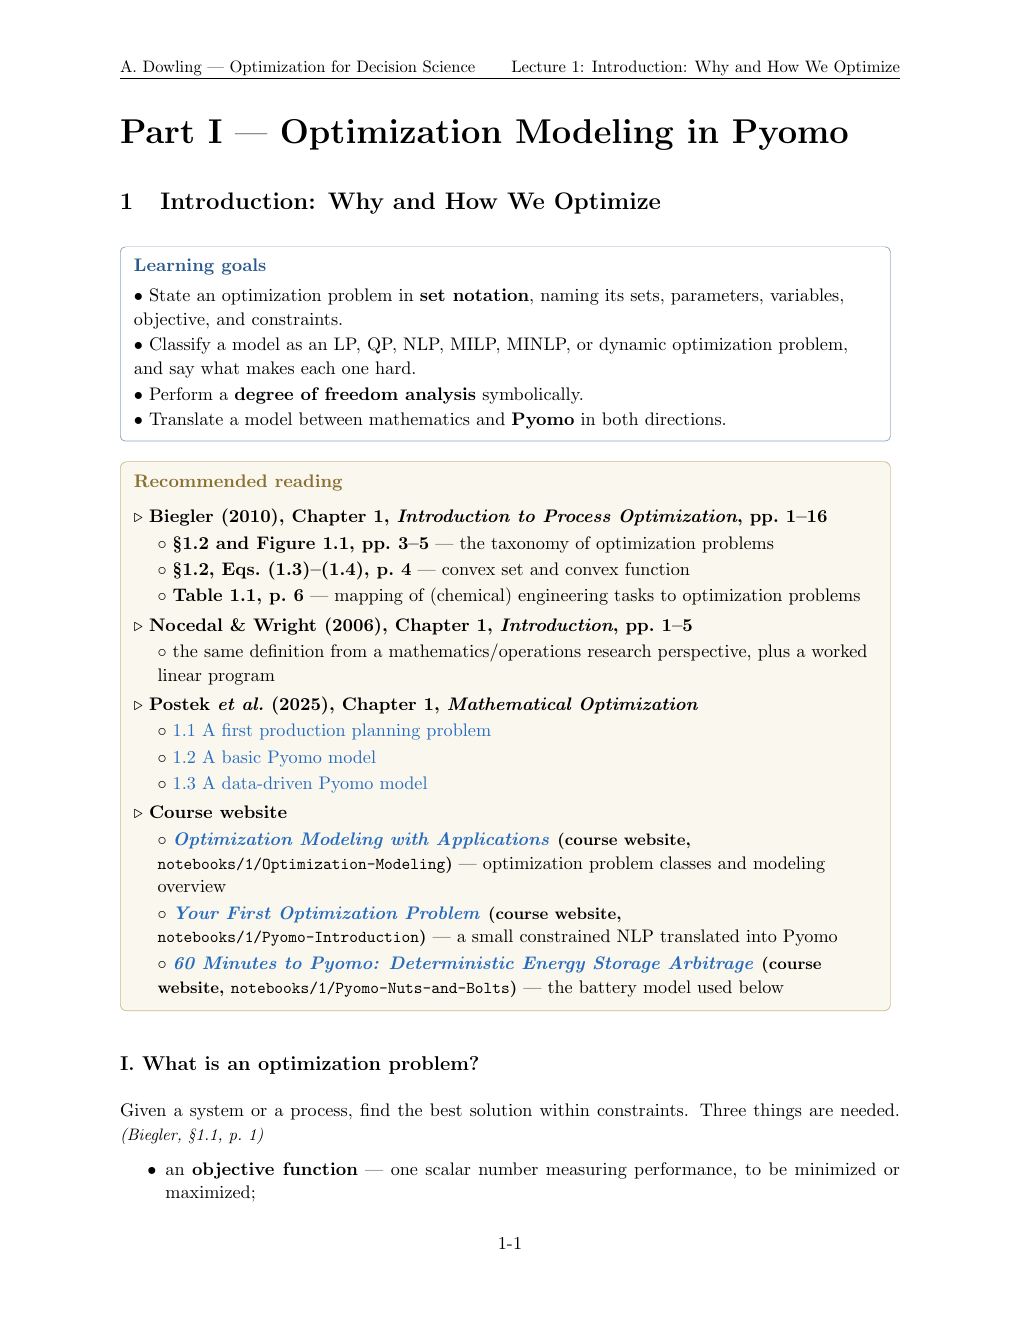
\includegraphics[width=0.98\linewidth,height=4.9cm,keepaspectratio,trim=65bp 185bp 70bp 270bp,clip]{figures/coursepack_sources.png}\\[0.4em]
      {\small Cross-references to literature\\and the course website}
    \end{column}
    \begin{column}{0.49\textwidth}
      \centering
      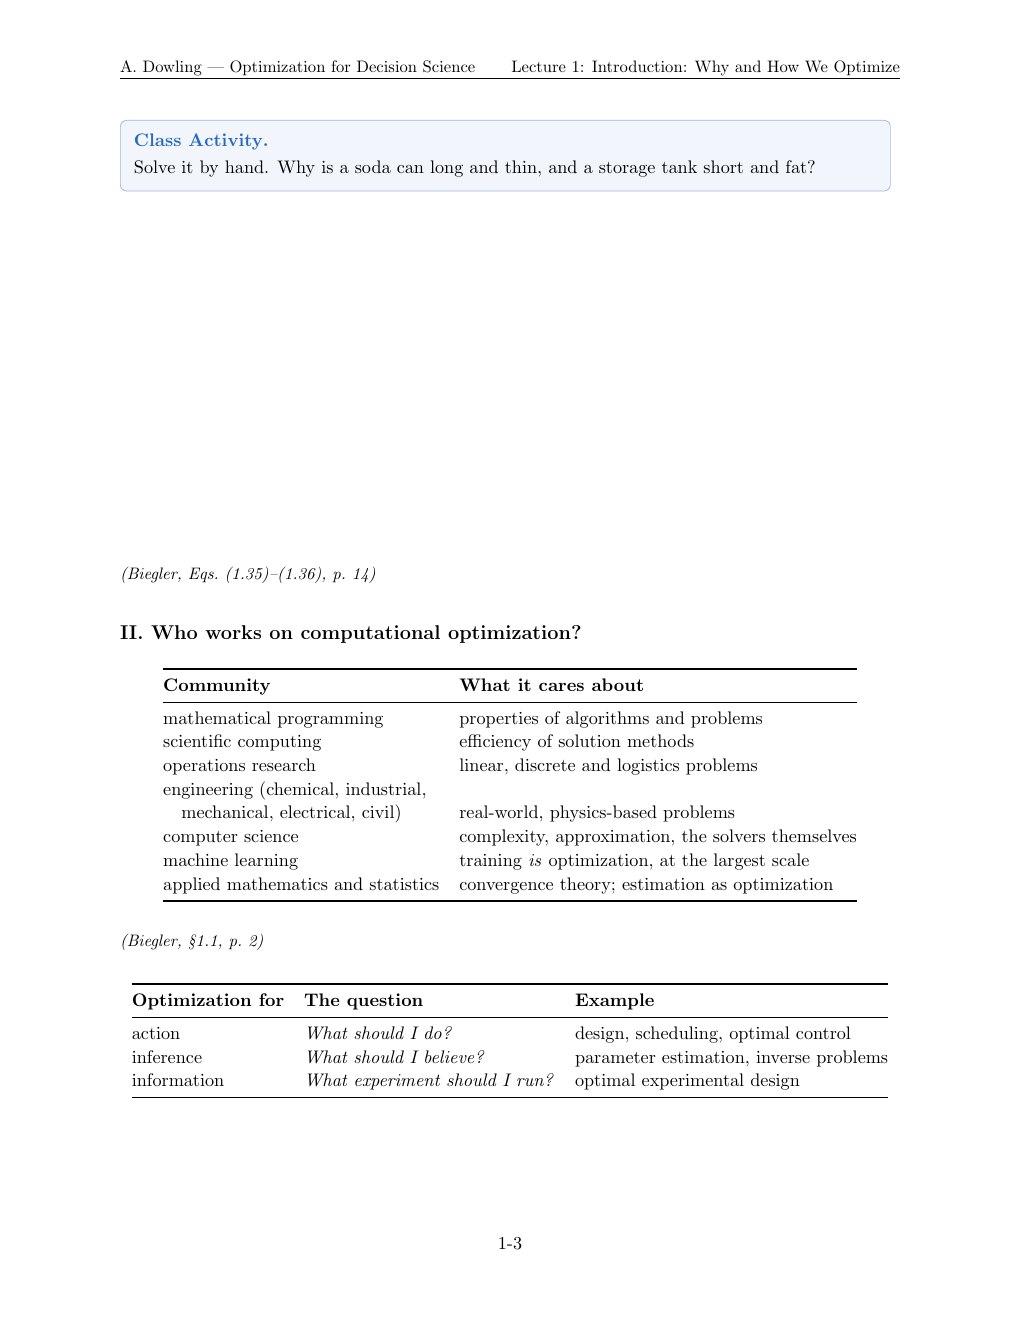
\includegraphics[width=0.98\linewidth,height=4.9cm,keepaspectratio,trim=65bp 420bp 70bp 50bp,clip]{figures/coursepack_gap.png}\\[0.4em]
      {\small Space for a derivation\\or discussion in class}
    \end{column}
  \end{columns}
  \vspace{0.5em}
  \begin{center}\small
    Students can trace the sources and work through the missing steps.
  \end{center}
  \vspace{0.45cm plus 1fill}
\end{frame}

\begin{frame}{Task 6: The course uses two repositories}
  \ndlogonote{\scriptsize\href{https://github.com/dowlinglab/claude-for-researchers/blob/main/resources/practices/scientific_computing_workflow.md}{\texttt{resources/practices/scientific\_computing\_workflow.md}}}
  \vfill
  \begin{columns}[t]
    \begin{column}{0.47\textwidth}
      \textbf{Authoritative sources}
      \begin{itemize}\small\setlength\itemsep{0.4em}
        \item \texttt{optimization-private}: lecture notes, coursepack, assessments
        \item \texttt{optimization}: notebooks, figure scripts, and data
      \end{itemize}
    \end{column}
    \begin{column}{0.47\textwidth}
      \textbf{Derived artifacts}
      \begin{itemize}\small\setlength\itemsep{0.4em}
        \item instructor, student, and alignment PDFs
        \item published notebooks, website, and figures
      \end{itemize}
    \end{column}
  \end{columns}
  \vspace{1.0em}
  \begin{center}\small
    A cross-repository solution-leak check enforces the private/public boundary.\\[0.35em]
    Claude and GPT helped map each goal to artifacts, then each likely failure to a test.
  \end{center}
  \vspace{1.0cm plus 1fill}
\end{frame}

\begin{frame}{Task 6: Each failure became a repeatable test}
  \ndlogonote{\scriptsize\href{https://github.com/dowlinglab/claude-for-researchers/blob/main/resources/scripts/check_docs.py}{\texttt{resources/scripts/check\_docs.py}}}
  \vfill
  \begin{center}\small
  \renewcommand{\arraystretch}{1.15}
  \begin{tabular}{@{}>{\raggedright\arraybackslash}p{4.6cm}>{\raggedright\arraybackslash}p{7.1cm}@{}}
    \toprule
    \textbf{Problem found} & \textbf{Test added} \\
    \midrule
    Missing citations & Resolve every key against \texttt{references.bib} \\
    Broken page layout & Render every page and check for clipping \\
    Notebook code drift & Compare notebook source across repos \\
    Solutions leaking into public files & Scan published notebooks for solutions \\
    Broken website routes & Rebuild the site and follow every internal link \\
    Stale figures & Re-execute figure scripts and compare outputs \\
    \bottomrule
  \end{tabular}
  \end{center}
  \vspace{0.6em}
  \begin{center}
    \slidepoint{Every recurring problem left a \textbf{mechanical test} behind.}
  \end{center}
  \vspace{0.45cm plus 1fill}
\end{frame}

\begin{frame}{Task 6: Git and handoffs bridge tools and computers}
  \ndlogonote{\scriptsize\href{https://github.com/dowlinglab/claude-for-researchers/blob/main/resources/checklists/reproducibility_and_handoff_checklist.md}{\texttt{resources/checklists/reproducibility\_and\_handoff\_checklist.md}}}
  \vfill
  \textbf{I switch between\ldots}
  \begin{itemize}\setlength\itemsep{0.35em}
    \item Claude and OpenAI tools
    \item my laptop and my desktop
    \item supervised and overnight sessions
  \end{itemize}
  \vspace{0.9em}
  \begin{enumerate}\setlength\itemsep{0.38em}
    \item The \textbf{goal document} defines phases, gates, safe decisions, and decisions reserved for me.
    \item Each agent commits a coherent change and updates the \textbf{handoff} with verified state.
    \item The next tool or computer reads the history and handoff, then reruns the relevant gate.
    \item I make pedagogical and scientific judgments. Agents inventory, edit, build, and check.
  \end{enumerate}
  \vfill
  \begin{center}
    \slidepoint{Git preserves state. Handoff documents preserve \textbf{intent and evidence}.}
  \end{center}
  \vspace{0.55cm plus 1fill}
\end{frame}

  
\stagedivider{5}{Epilogue: Trust}{What do you trust, and why?}

\begin{frame}{Currently, Claude is approved for public data only at ND}
  \vfill
  \renewcommand{\arraystretch}{0.9}
  \begin{center}
  \begin{tabular}{@{}lll@{}}
    \toprule
    \textbf{Tier} & \textbf{Examples} & \textbf{AI use} \\
    \midrule
    \textcolor{OkGreen}{$\bullet$}~Public    & published, press-released & safe \\
    \textcolor{NDGold!80!black}{$\bullet$}~Internal  & routine business data & safe \emph{in approved tools} \\
    \textcolor{OkVermillion}{$\bullet$}~Sensitive & role-restricted       & safe \emph{in approved tools} \\
    \textcolor{black}{$\blacksquare$}~Restricted & SSN, health, payment  & \bad{never, in any tool} \\
    \bottomrule
  \end{tabular}
  \end{center}
  \vspace{0.5em}
  \begin{center}
  \begin{tabular}{@{}lc@{}}
    \toprule
    \textbf{Tool} & \textbf{Approved through} \\
    \midrule
    Gemini, ChatGPT EDU, NotebookLM & Sensitive \\
    \textbf{Claude} & \textbf{Public only} \\
    \bottomrule
  \end{tabular}
  \end{center}
  \renewcommand{\arraystretch}{1}
  \vspace{0.5em}
  \begin{center}
    \small Claude Team accounts (free for academic labs) do not train on your data by default, but have a risk/reward conversation with your PI.
  \end{center}
  \vspace{0.55cm plus 1fill}
\end{frame}

\begin{frame}{Two important notes}
  \vfill
  \begin{itemize}\setlength\itemsep{1.2em}
    \item \textbf{DoD / DoW funding?}\\
      Certain funding agencies currently \bad{prohibit}
      using any Anthropic product --- Claude.ai, the API, Claude
      Code.\\[0.3em]
      {\small Questions: \texttt{researchsecurity@nd.edu} (CC your PI)}
    \item \textbf{Everyone else: ask your PI.}\\
      Export control, sponsor terms, intellectual property protection, and IRB conditions differ per
      project
  \end{itemize}
  \vfill
\end{frame}

\begin{frame}{The six tasks form one research workflow}
  \vfill
  \begin{center}
  \small\setlength{\tabcolsep}{4pt}
  \begin{tabular}{@{}llccccc@{}}
    \toprule
    & & \textbf{Prologue} & \textbf{Act I} & \textbf{Act II} & \textbf{Act III} \\
    \midrule
    \textbf{\color{NDGold!80!black}Part 1} & Task 1 --- set up agents + inherit a project & & \good{} & & \\
    & Task 2 --- paper code $\to$ package & \good{} & & \good{} & \\
    \midrule
    \textbf{\color{NDGold!80!black}Part 2} & Task 3 --- idea $\to$ literature review, report, or proposal & & & \good{} & \\
    & Task 4 --- audit a manuscript & & & & \good{} \\
    & Task 5 --- project $\to$ manuscript & & & & \good{} \\
    & Task 6 --- modernize a course & & & & \good{} \\
    \bottomrule
  \end{tabular}
  \end{center}
  \vfill
  \begin{center}
    The later tasks reuse the repository, environment, corpus, and checks established earlier.
  \end{center}
  \vfill
\end{frame}

\begin{frame}{This talk was built with the practices it recommends}
  \ndlogonote{\scriptsize\href{https://github.com/dowlinglab/ND_Beamer_Template}{\texttt{github.com/dowlinglab/ND\_Beamer\_Template}}}
  \vspace{-0.3cm}
  \begin{enumerate}\setlength\itemsep{0.6em}
    \item Identified 10+ AI-accelerated projects from the past year
    \item Dispatched agents to examine each project's full history
    \item Distilled the findings into actionable practice guides
    \item Crafted a story arc and outline
    \item Built these slides iteratively with Claude and GPT
      \begin{itemize}\small\setlength\itemsep{0.2em}
        \item Claude analyzed my past talks to match my style
        \item I made the editorial decisions
      \end{itemize}
  \end{enumerate}
  \vfill
\end{frame}

\begin{frame}{You own every claim, whatever helped you make it}
  \vfill
  \begin{itemize}\setlength\itemsep{0.9em}
    \item AI drafts, checks, and challenges. It does not decide what's true.
    \item Disclose AI use the way you'd disclose a collaborator's contribution --- journals increasingly expect it named as a research method, not left in a footnote.
    \item I checked factual claims against primary evidence before they went on a slide. Personal estimates remain labeled as such.
    \item The same standard applies to your own work, whatever helped you produce it.
  \end{itemize}
  \vfill
\end{frame}

\begin{frame}{Hobbies: AI can amplify your curiosity}
  \vspace{0.02cm plus 1fill}
  \begin{columns}[c]
    \begin{column}{0.48\textwidth}
      \centering
      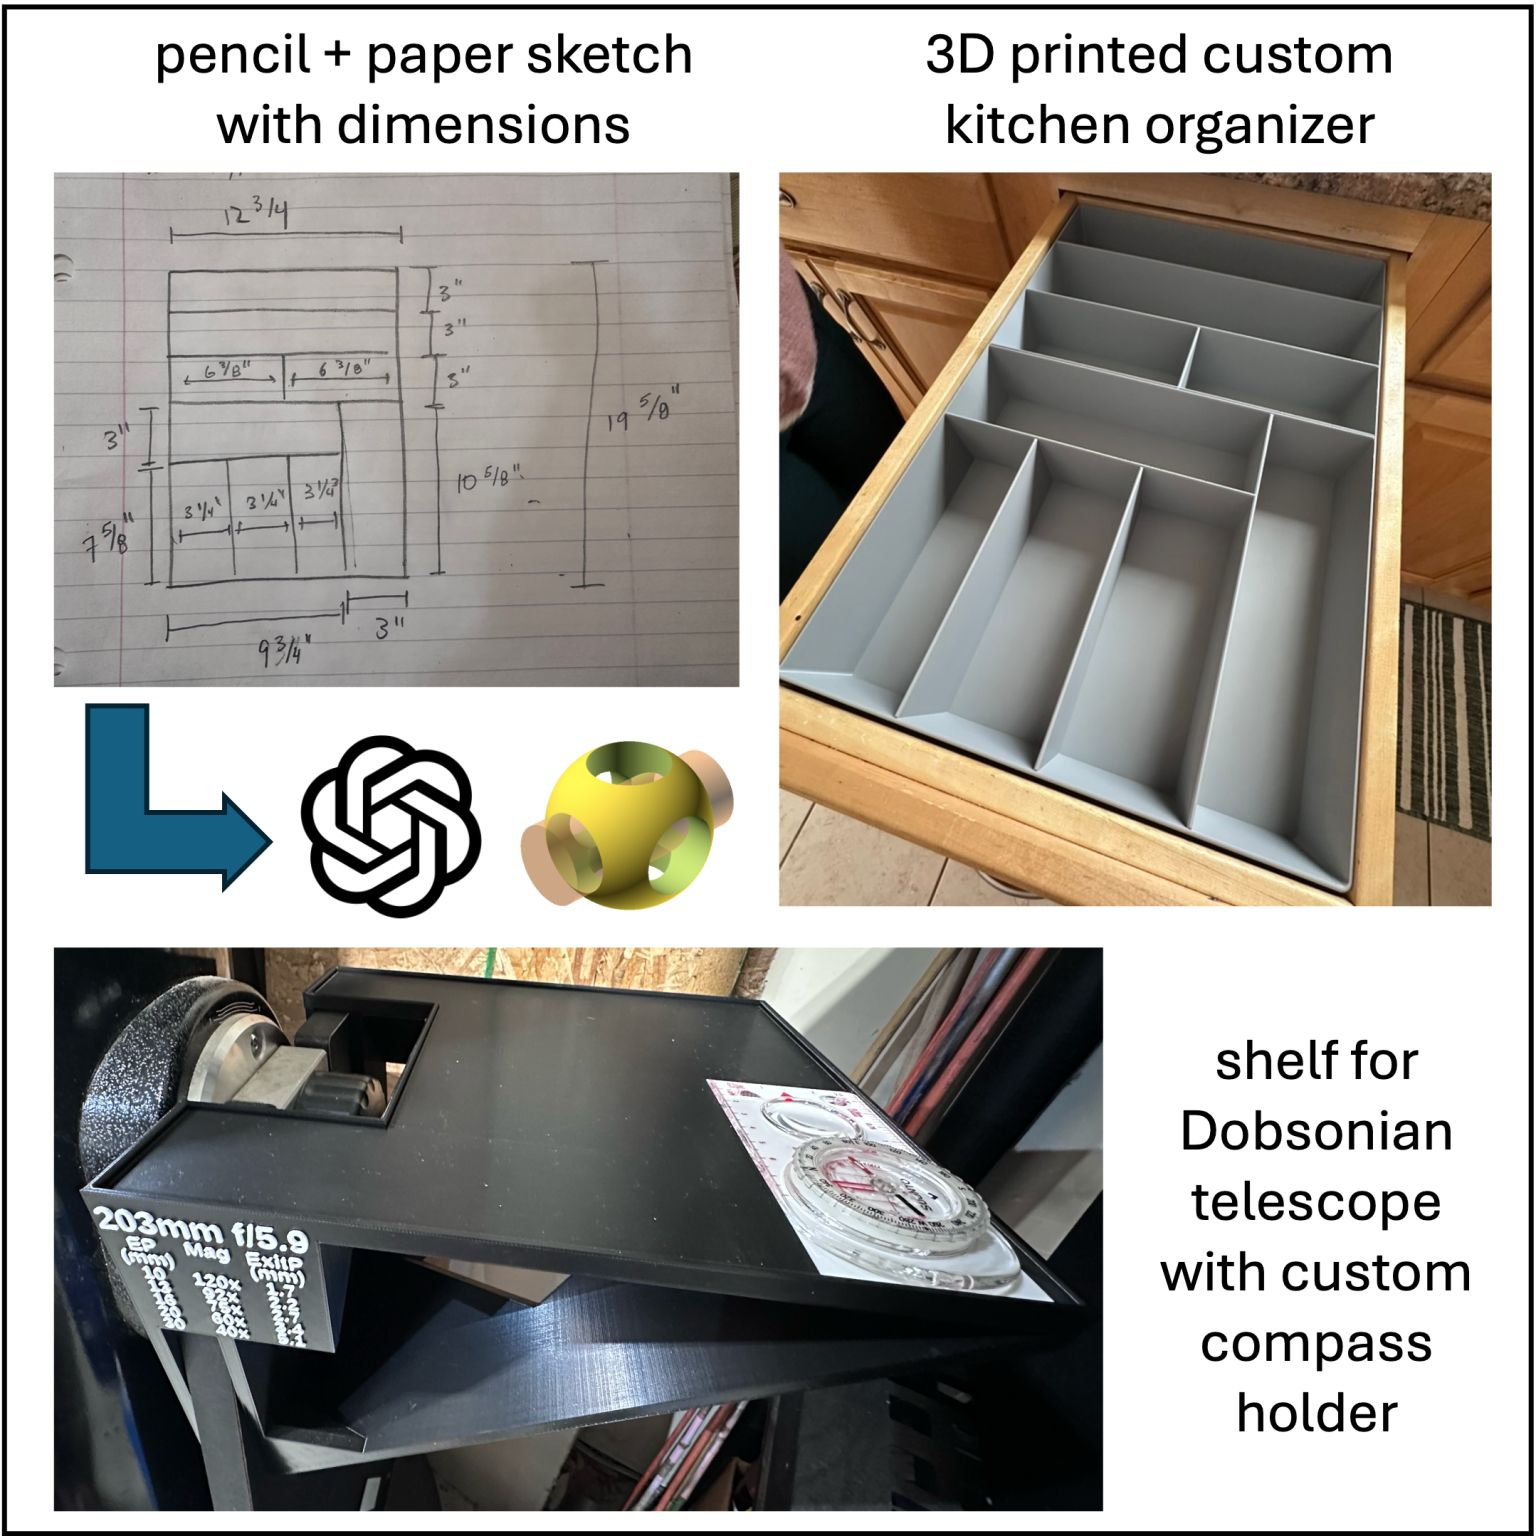
\includegraphics[height=5.75cm]{figures/kitchen_organizer_telescope_shelf.jpeg}
    \end{column}
    \begin{column}{0.46\textwidth}
      \textbf{\small My workflow}
      \begin{enumerate}\small\setlength\itemsep{0.05em}
        \item Sketch on paper, or lately, photos with a tape measure/caliper
        \item \texttt{init\_project.sh}; design in OpenSCAD, iterating with Codex against \texttt{STYLE.md}
        \item \texttt{render\_views.sh} for views --- falls back to Blender on OpenSCAD crashes
        \item Look at the views, tell Codex what's wrong, repeat until it matches the sketch
      \end{enumerate}
      \vspace{0.1em}
      \textbf{\small Projects}
      \begin{itemize}\small\setlength\itemsep{0.05em}
        \item organizers, telescope shelf and caps
        \item camera mounts, keychains, tablet mount
      \end{itemize}
    \end{column}
  \end{columns}
  \vspace{0.15cm plus 1fill}
\end{frame}

\begin{frame}{Hobbies: Create a textbook customized for you}
  \ndlogonote{\scriptsize\href{https://github.com/adowling2/radio-extra-book}{\texttt{github.com/adowling2/radio-extra-book}}}
  \vspace{0.1cm}
  \begin{center}
    I used Claude to create a \textbf{personalized textbook}: learn AC circuit theory for the \textbf{amateur radio license exam}.
  \end{center}
  \vspace{0.35em}
  \begin{columns}[c]
    \begin{column}{0.40\textwidth}
      \textbf{\small My approach}
      \begin{enumerate}\small\setlength\itemsep{0.1em}
        \item Connect circuit theory to my background with ChatGPT
        \item Draft the source, chapter by chapter
        \item Organize the chapters into parts
        \item Build a reproducible figure pipeline
        \item Check coverage against the exam pool
        \item Revise in structured rounds
      \end{enumerate}
    \end{column}
    \begin{column}{0.56\textwidth}
      \centering
      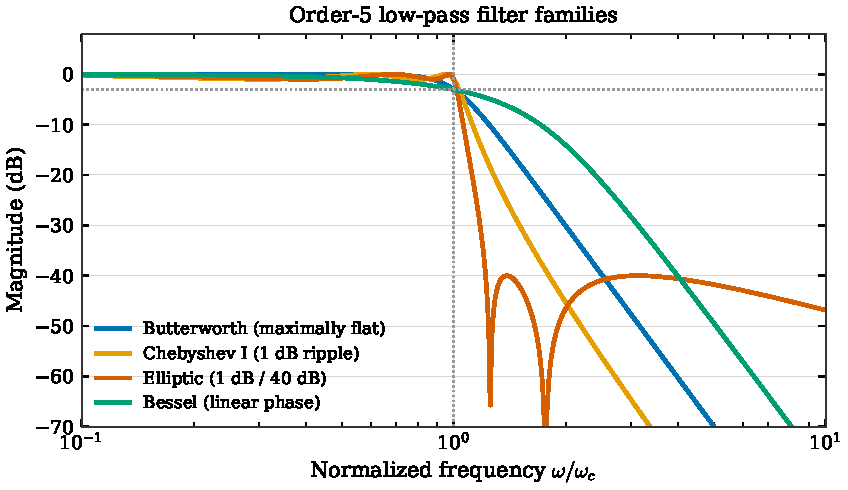
\includegraphics[width=0.8\linewidth]{figures/filter_families}\\[0.05em]
      {\scriptsize Example: understand how low-pass filters differ.}
    \end{column}
  \end{columns}
  \vspace{0.95cm plus 1fill}
\end{frame}


\begin{frame}[fragile]{Going from workshop activities to research workflows}
  \ndlogonote{\scriptsize\href{https://github.com/dowlinglab/claude-for-researchers}{\texttt{github.com/dowlinglab/claude-for-researchers}}}
  \vfill
  \begin{enumerate}\small\setlength\itemsep{0.5em}
    \item Clone this repo with \textbf{GitHub Desktop} and explore it with an agent.
    \item Use the \textbf{getting-started prompt} to connect the resources to your research.
  \end{enumerate}
  \vspace{0.4em}
  \begin{lstlisting}[basicstyle=\ttfamily\small]
Explore this repository and explain its main resources.
Then use "The prompt" in resources/prompts/getting_started.md
to interview me about my research and recommend where to start.
Do not edit any files yet.
  \end{lstlisting}
  \begin{center}\small
    Choose Claude or ChatGPT, whichever you prefer.\\[0.3em]
    \href{https://github.com/dowlinglab/claude-for-researchers/blob/main/resources/prompts/getting_started.md}{\texttt{resources/prompts/getting\_started.md}}
  \end{center}
  \vspace{0.8cm plus 1fill}
\end{frame}

  \begin{frame}{Part 2 Activity: A teammate hands you a folder}
  \vfill
  \begin{center}
    \resizebox{0.98\linewidth}{!}{\begin{tikzpicture}[font=\large\sffamily, >=Stealth]
      \node[nd box, minimum width=4.2cm, minimum height=1.6cm] (d) at (0,0) {\textbf{Data}\\{\small \texttt{data/penguins.csv}}};
      \node[nd box, minimum width=4.2cm, minimum height=1.6cm] (n) at (5.4,0) {\textbf{Notebook}\\{\small code and saved outputs}};
      \node[nd highlight, minimum width=4.2cm, minimum height=1.6cm] (w) at (10.8,0) {\textbf{Write-up}\\{\small \texttt{writeup.md}: the claims}};
      \node[nd box, minimum width=4.2cm, minimum height=1.6cm] (f) at (5.4,-2.3) {\textbf{Figures}\\{\small two PNG files}};
      \node[nd box, minimum width=4.2cm, minimum height=1.6cm] (r) at (10.8,-2.3) {\textbf{References}\\{\small open texts to check against}};
      \draw[->, very thick, NDBlue] (d) -- (n);
      \draw[->, very thick, NDBlue] (n) -- (w);
      \draw[->, very thick, NDBlue] (n) -- (f);
      \draw[->, very thick, NDBlue] (f) -- (w);
      \draw[->, very thick, NDBlue, dashed] (r) -- (w);
    \end{tikzpicture}}
  \end{center}
  \vspace{0.8em}
  \begin{center}
    \slidepoint{Every claim in the write-up should trace back to the \textbf{data}, the \textbf{notebook}, or a \textbf{reference}.}
  \end{center}
  \vspace{1.6cm plus 1fill}
\end{frame}

\begin{frame}[fragile]{The data: Palmer Penguins}
  \vfill
  \begin{lstlisting}[basicstyle=\ttfamily\scriptsize, breaklines=false]
species,island,bill_length_mm,bill_depth_mm,flipper_length_mm,body_mass_g,sex,year
Adelie,Torgersen,39.1,18.7,181,3750,male,2007
Adelie,Torgersen,39.5,17.4,186,3800,female,2007
Adelie,Torgersen,40.3,18,195,3250,female,2007
...
  \end{lstlisting}
  {\small \texttt{data/penguins.csv}: one row per penguin, with bill, flipper, body mass, and sex measurements}\\[1.0em]
  \begin{center}
    \begin{tikzpicture}[font=\sffamily]
      \node[nd box, minimum width=3.1cm, minimum height=1.7cm] at (-4.8,0) {{\LARGE\textbf{344}}\\{\small penguins}};
      \node[nd box, minimum width=3.1cm, minimum height=1.7cm] at (-1.6,0) {{\LARGE\textbf{3}}\\{\small species}};
      \node[nd box, minimum width=3.1cm, minimum height=1.7cm] at (1.6,0) {{\LARGE\textbf{3}}\\{\small islands}};
      \node[nd box, minimum width=3.1cm, minimum height=1.7cm] at (4.8,0) {{\LARGE\textbf{2007--09}}\\{\small public data (CC0)}};
    \end{tikzpicture}
  \end{center}
  \vspace{1.5cm plus 1fill}
\end{frame}

\begin{frame}{The notebook: text, code, and saved outputs}
  \vfill
  \begin{center}
    \fbox{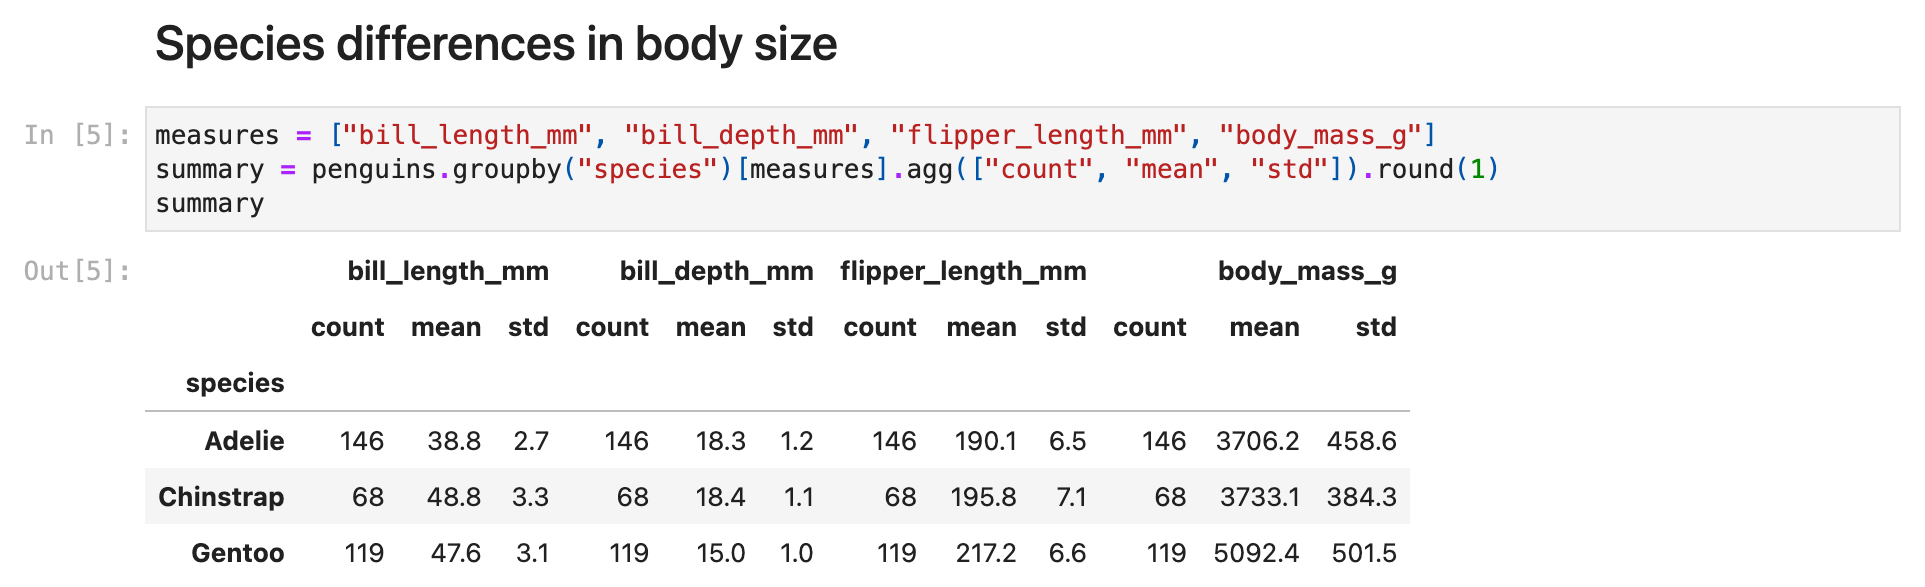
\includegraphics[width=0.78\linewidth]{figures/penguin_notebook_excerpt.png}}\\[0.7em]
    \begin{tikzpicture}[font=\small\sffamily]
      \node[nd box, text width=3.9cm, minimum height=1.4cm, inner sep=5pt] at (-4.4,0) {\textbf{Text cells}\\explain the analysis};
      \node[nd box, text width=3.9cm, minimum height=1.4cm, inner sep=5pt] at (0,0) {\textbf{Code cells}\\numbered, like \texttt{In [5]}};
      \node[nd highlight, text width=3.9cm, minimum height=1.4cm, inner sep=5pt] at (4.4,0) {\textbf{Saved outputs}\\like \texttt{Out [5]}: no need to run};
    \end{tikzpicture}
  \end{center}
  \vspace{1.5cm plus 1fill}
\end{frame}

\begin{frame}{The notebook's analysis, section by section}
  \vfill
  \begin{columns}[c]
    \begin{column}{0.58\textwidth}
      \begin{enumerate}\large\setlength\itemsep{0.5em}
        \item Load and clean
        \item Species differences in body size
        \item Flipper length: Adelie vs Chinstrap
        \item Body mass and sex in Adelie penguins
        \item Differences among islands
        \item Bill length and bill depth
        \item Figure 1
      \end{enumerate}
    \end{column}
    \begin{column}{0.38\textwidth}
      \slidepoint{Summary tables, \textbf{statistical tests}, and two figures.}
    \end{column}
  \end{columns}
  \vspace{1.5cm plus 1fill}
\end{frame}

\begin{frame}[fragile]{The write-up: the claims you will check}
  \vfill
  \begin{columns}[c]
    \begin{column}{0.62\textwidth}
      \begin{lstlisting}[basicstyle=\ttfamily\footnotesize, breaklines=false]
# Body size in three Palmer Archipelago
  penguin species
## 1. Data and methods
## 2. Species differ in body mass
## 3. Flipper length differs between
     Adelie and Chinstrap penguins
## 4. Sex differences in Adelie body mass
## 5. Island effects
## 6. Bill shape
## 7. Figure
## 8. Conclusions
## References
      \end{lstlisting}
      {\small \texttt{writeup.md}: draft results for a group meeting}
    \end{column}
    \begin{column}{0.34\textwidth}
      \textbf{It makes claims:}
      \begin{itemize}\large\setlength\itemsep{0.5em}
        \item numbers
        \item comparisons
        \item interpretations
        \item conclusions
      \end{itemize}
    \end{column}
  \end{columns}
  \vspace{1.5cm plus 1fill}
\end{frame}

\begin{frame}{The figures saved by the notebook}
  \vfill
  \begin{center}
    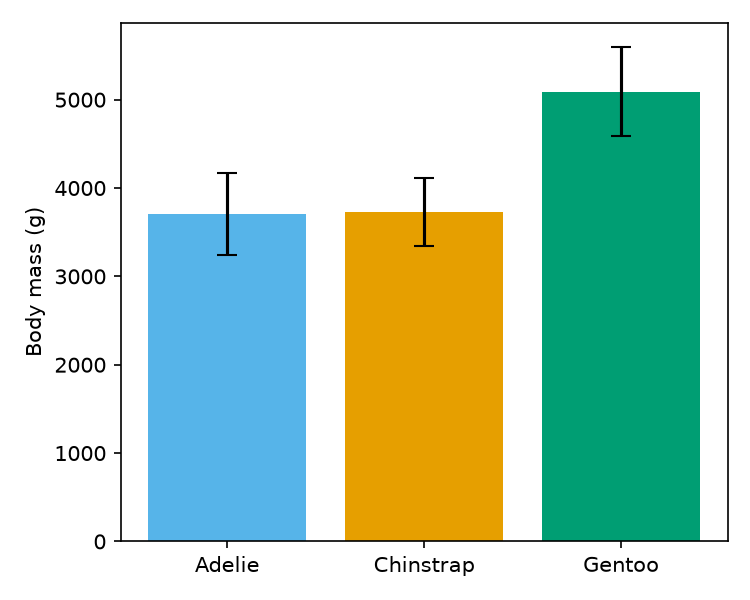
\includegraphics[height=4.9cm]{figures/penguin_body_mass_by_species.png}\hspace{0.8cm}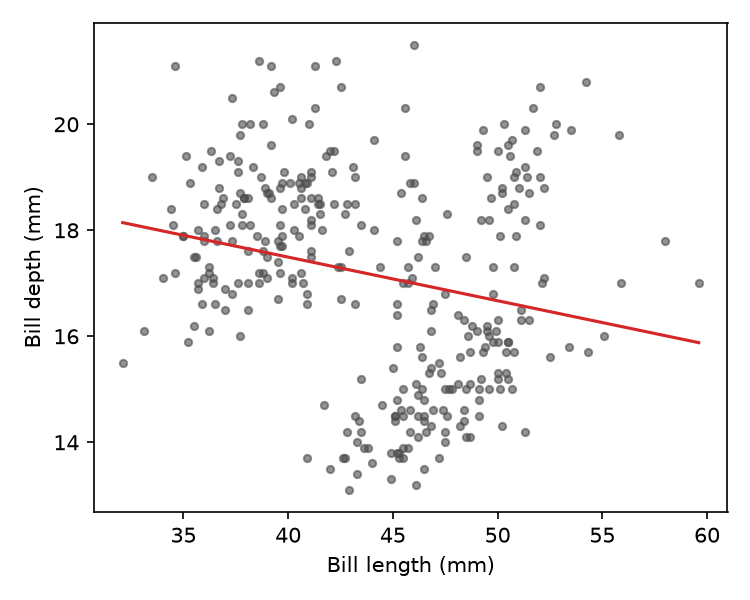
\includegraphics[height=4.9cm]{figures/penguin_bill_length_vs_depth.png}\\[0.5em]
    {\small \texttt{figures/}: two PNG files, one used in the write-up}
  \end{center}
  \vspace{1.5cm plus 1fill}
\end{frame}

\begin{frame}{Activity 2: check a teammate's analysis with an LLM}
  \vfill
  \begin{columns}[c]
    \begin{column}{0.50\textwidth}
      \resizebox{\linewidth}{!}{\begin{tikzpicture}[font=\small\sffamily, >=Stealth]
        \node[nd box, minimum width=4.2cm, minimum height=1.2cm] (a) at (0,1.7) {\textbf{Notebook}\\{\footnotesize with saved outputs}};
        \node[nd box, minimum width=4.2cm, minimum height=1.2cm] (b) at (0,0) {\textbf{Write-up}\\{\footnotesize the claims}};
        \node[nd box, minimum width=4.2cm, minimum height=1.2cm] (c) at (0,-1.7) {\textbf{Reference texts}\\{\footnotesize open statistics sources}};
        \node[nd highlight, minimum width=3.4cm, minimum height=2.4cm] (d) at (6.4,0) {\textbf{An audit}\\{\footnotesize that you}\\{\footnotesize have checked}};
        \draw[->, very thick, NDBlue] (a.east) -- (d.north west);
        \draw[->, very thick, NDBlue] (b.east) -- (d.west);
        \draw[->, very thick, NDBlue] (c.east) -- (d.south west);
      \end{tikzpicture}}
    \end{column}
    \begin{column}{0.46\textwidth}
      \slidepoint{A member of your team gives you \textbf{this notebook} with a statistical analysis.}\\[0.9em]
      {\small How can you use an LLM to \textbf{augment your critical thinking} and check the analysis?}\\[0.9em]
      {\small It contains deliberate problems, some easy and some subtle. We will not say how many.}\\[0.7em]
      {\small Pick up the \textbf{Part 2 handout} and turn to the activity on the back.}
    \end{column}
  \end{columns}
  \vfill
  \ndlogonote{\scriptsize Hands-on: 45 minutes; regroup: 15 minutes}
\end{frame}

\begin{frame}{The setup: the data, the questions, and what to check against}
  \vfill
  \begin{center}
    \begin{tikzpicture}[font=\small\sffamily]
      \node[nd box, text width=0.27\textwidth, minimum height=4.3cm, align=left, inner sep=8pt, anchor=north] at (-0.325\textwidth,0)
        {\textbf{\normalsize The data}\\[0.4em]
         Palmer Penguins\\
         344 penguins, 3 species, 3 islands, 2007--2009\\[0.4em]
         {\footnotesize Bill length and depth, flipper length, body mass, sex\\[0.2em] Public, CC0}};
      \node[nd box, text width=0.27\textwidth, minimum height=4.3cm, align=left, inner sep=8pt, anchor=north] at (0,0)
        {\textbf{\normalsize The questions}\\[0.4em]
         How do the species differ in size?\\[0.3em]
         Do males and females differ?\\[0.3em]
         Do the islands matter?\\[0.3em]
         How are bill length and depth related?};
      \node[nd highlight, text width=0.27\textwidth, minimum height=4.3cm, align=left, inner sep=8pt, anchor=north] at (0.325\textwidth,0)
        {\textbf{\normalsize To check against}\\[0.4em]
         Three open references:\\
         {\footnotesize a statistics textbook, the NIST e-Handbook, the ASA statement on p-values}\\[0.4em]
         The raw data file and its documentation};
    \end{tikzpicture}
  \end{center}
  \vspace{0.6em}
  \begin{center}
    \slidepoint{Decide which claims you would let \textbf{stand}.}
  \end{center}
  \vspace{1.6cm plus 1fill}
\end{frame}

\begin{frame}[fragile]{Get the materials and open the folder in Claude}
  \vfill
  \begin{columns}[c]
    \begin{column}{0.48\textwidth}
      \begin{enumerate}\small\setlength\itemsep{0.6em}
        \item \href{https://github.com/dowlinglab/claude-for-researchers/releases/latest}{\textbf{Download the ZIP}} (address below) and unzip it.
        \item Open the \texttt{audit-project} folder itself in Claude. In a chat app, attach \texttt{writeup.md}, the notebook, and \texttt{data/README.md}.
        \item Paste the \textbf{starter prompt} on the next slide. It includes the reference links.
        \item \textbf{Optional:} save a reference copy in \texttt{references/pdfs/}. If Claude cannot find it, tell it the file name.
      \end{enumerate}
    \end{column}
    \begin{column}{0.50\textwidth}
      \begin{lstlisting}[basicstyle=\ttfamily\scriptsize]
audit-project/
  writeup.md         the claims
  notebooks/         the analysis
  data/              data and README
  figures/           two figures
  references/pdfs/   optional copies
  environment.yml    optional
      \end{lstlisting}
    \end{column}
  \end{columns}
  \vspace{0.4em}
  \begin{center}
    {\small\href{https://github.com/dowlinglab/claude-for-researchers/releases/latest}{\texttt{github.com/dowlinglab/claude-for-researchers/releases/latest}}, under \textbf{Assets}}
  \end{center}
  \vspace{1.6cm plus 1fill}
\end{frame}

\begin{frame}{Start with a prompt that reads before it judges}
  \vfill
  \begin{center}
    \begin{tikzpicture}
      \node[nd box, text width=0.92\linewidth, inner sep=8pt, align=left, font=\small] {\hyphenpenalty=10000\relax
        A teammate sent me this notebook and write-up. I want to audit the analysis, not fix it. Read the write-up, the notebook, and the data documentation, and change nothing. List each substantive claim and where it appears. Then give each claim a status (supported, questionable, incorrect, or insufficient evidence). Say whether you checked it against the notebook's output, the raw data, or a reference, cite the section you relied on, and tell me what you could not open or check. References: the files in \texttt{references/pdfs/}, or these links: \texttt{openintro-ims.netlify.app}, \texttt{itl.nist.gov/div898/handbook}, \texttt{amstat.org/asa/files/pdfs/p-valuestatement.pdf}.};
    \end{tikzpicture}
  \end{center}
  \vspace{0.5em}
  \begin{center}
    \slidepoint{Ask for the \textbf{evidence} and its \textbf{location}, not just a verdict.}\\[0.4em]
    {\small One message covers Steps 1 to 3. Edit it freely, and ask what any unfamiliar term means.}
  \end{center}
  \vspace{1.6cm plus 1fill}
\end{frame}

\begin{frame}{Ask, inspect, verify, iterate}
  \vfill
  \begin{center}
    \resizebox{0.94\linewidth}{!}{\begin{tikzpicture}[font=\normalsize\sffamily, >=Stealth]
      \node[nd box, minimum width=3.4cm, minimum height=2.3cm] (n1) at (0,0) {\textbf{Ask}\\[2pt]{\footnotesize list the claims,}\\{\footnotesize check them against}\\{\footnotesize the references}};
      \node[nd box, minimum width=3.4cm, minimum height=2.3cm] (n2) at (4.4,0) {\textbf{Inspect}\\[2pt]{\footnotesize read every finding}\\{\footnotesize and where it points}};
      \node[nd highlight, minimum width=3.4cm, minimum height=2.3cm] (n3) at (8.8,0) {\textbf{Verify}\\[2pt]{\footnotesize open the reference,}\\{\footnotesize recompute the number}};
      \node[nd box, minimum width=3.4cm, minimum height=2.3cm] (n4) at (13.2,0) {\textbf{Iterate}\\[2pt]{\footnotesize sharpen the prompt,}\\{\footnotesize add context, repeat}};
      \foreach \a/\b in {1/2, 2/3, 3/4} { \draw[->, very thick, NDBlue] (n\a) -- (n\b); }
    \end{tikzpicture}}
  \end{center}
  \vspace{1.1em}
  \begin{center}
    \bad{Prompt $\rightarrow$ trust $\rightarrow$ done}\\[0.9em]
    {\small Ask for a status on every claim: supported, questionable, incorrect, or insufficient evidence.}
  \end{center}
  \vspace{1.4cm plus 1fill}
\end{frame}
\begin{frame}{Give every claim one of four statuses}
  \vfill
  \renewcommand{\arraystretch}{1.5}
  \begin{center}
    \small
    \begin{tabular}{@{}p{3.2cm}p{9.2cm}@{}}
      \toprule
      \textbf{Status} & \textbf{Use it when}\\
      \midrule
      Supported & The notebook's output, the data, or a cited reference agrees. Ask which.\\
      Questionable & The claim may hold, but the wording or method is doubtful.\\
      Incorrect & The evidence or a cited reference contradicts the claim.\\
      Insufficient evidence & These files cannot show it either way. This is not the same as wrong.\\
      \bottomrule
    \end{tabular}
  \end{center}
  \vspace{0.8em}
  \begin{center}
    \slidepoint{\textbf{Insufficient evidence} is a result, not a failure.}
  \end{center}
  \vspace{1.6cm plus 1fill}
\end{frame}

\begin{frame}[fragile]{Optional Step 0: make agent changes easy to review}
  \vfill
  \begin{columns}[c]
    \begin{column}{0.44\textwidth}
      {\small\textbf{Optional, if you are comfortable with Git and Python.}\\
      If not, skip it. You are not behind.}\\[0.8em]
      \begin{enumerate}\small\setlength\itemsep{0.35em}
        \item Commit a clean \textbf{baseline} before anything changes.
        \item Move the analysis code into readable \textbf{Python files}.
        \item Commit the refactor \textbf{separately}.
        \item Then start the audit.
      \end{enumerate}
    \end{column}
    \begin{column}{0.54\textwidth}
      {\footnotesize\textbf{Notebook:} change one number, rerun}
      \begin{lstlisting}[basicstyle=\ttfamily\scriptsize, aboveskip=0.1em, belowskip=0.2em]
- "image/png": "iVBOR..." [34,731 chars]
+ "image/png": "iVBOR..." [35,271 chars]
- "ax.scatter(...\"depth\"], s=12,...
+ "ax.scatter(...\"depth\"], s=16,...
      \end{lstlisting}
      {\footnotesize\textbf{Python file:} the same change}
      \begin{lstlisting}[basicstyle=\ttfamily\scriptsize, aboveskip=0.1em, belowskip=0.2em]
-  ax.scatter(x, y, s=12, alpha=0.6)
+  ax.scatter(x, y, s=16, alpha=0.6)
      \end{lstlisting}
    \end{column}
  \end{columns}
  \vspace{0.3em}
  \begin{center}\small
    The right format depends on the task. For heavy agent editing, plain text is easier to audit.
  \end{center}
  \vspace{0.6cm plus 1fill}
\end{frame}
\begin{frame}{Then judge the audit itself}
  \vfill
  \begin{columns}[c]
    \begin{column}{0.50\textwidth}
      \slidepoint{Keep a \textbf{log}: finding, evidence, how you checked it.}\\[0.9em]
      {\small Verify at least \textbf{three} findings yourself: a number, a citation, and a claim marked \emph{Supported}.}\\[0.6em]
      {\small Note which model and setup you used.}\\[0.6em]
      {\small Save your log at minute 40.}
    \end{column}
    \begin{column}{0.46\textwidth}
      \begin{itemize}\small\setlength\itemsep{0.55em}
        \item What did it find, and what did it miss?
        \item Did it invent anything?
        \item Were its citations accurate?
        \item What improved it?
      \end{itemize}
    \end{column}
  \end{columns}
  \vspace{1.4cm plus 1fill}
\end{frame}

  \begin{frame}{Regroup 2: how good was the audit?}
  \vfill
  \begin{center}
    \slidepoint{How many problems did Claude (or Codex) \textbf{find}, and how many did \textbf{you verify}?}\\[1.1em]
    {\small What did it miss? Did it report anything that was not a problem?}\\[0.8em]
    {\small Which \textbf{model and setup} did you use? Did the choice change the audit?}\\[0.8em]
    {\small Which prompt or added context improved it? Were its citations accurate?}\\[1.1em]
    {\small Take one audit habit back to your own research.}
  \end{center}
  \vfill
  \ndlogonote{\scriptsize Regroup: 15 minutes; participants share first}
\end{frame}

  \parttworegroup
  \begin{frame}{Give feedback, then keep learning with SAI Sparks}
  \vfill
  \begin{center}
    \begin{tikzpicture}
      \node[nd highlight, inner sep=0.22cm, text width=5.6cm] (survey) {%
        {\large\textbf{Workshop feedback}}\\[0.35em]
        \qrcode[height=3.0cm]{https://forms.gle/RMcpwBSG3GP9fF1u5}\\[0.35em]
        {\small\href{https://forms.gle/RMcpwBSG3GP9fF1u5}{\texttt{forms.gle/RMcpwBSG3GP9fF1u5}}}\\[0.3em]
        {\small What helped? What should change? What should we cover next?}};
      \node[nd box, inner sep=0.22cm, text width=5.6cm, right=0.9cm of survey] {%
        {\large\textbf{SAI Sparks tutorials}}\\[0.35em]
        \qrcode[height=3.0cm]{https://sai.nd.edu/programs/sai-sparks/}\\[0.35em]
        {\small\href{https://sai.nd.edu/programs/sai-sparks/}{\texttt{sai.nd.edu/programs/sai-sparks}}}\\[0.3em]
        {\small Weekly hands-on AI tutorials for graduate students and postdocs.}};
    \end{tikzpicture}
  \end{center}
  \vspace{1.5cm plus 1fill}
\end{frame}

\fi

\end{document}
